\chapter{دراسة نظرية ومرجعية}
\section{مقدمة}
يعرض هذا الفصل مقدمة عن مفهوم الملاحقة وعن أنواعها، بالإضافة إلى دراسة مرجعية بأنواع خوارزميات الملاحقة فيما يخص التعلم العميق، ثم ننتقل إلى شرح نموذج المحول كونه الكتلة الأساسية في خوارزمية الملاحقة 
\textLR{SwinTrack\cite{swinTrack}},
بحيث نبدأ بشرح عام عن النماذج السابقة له، وكيفية تطور بنيته، ونعرض بالتفصيل تابع الانتباه وهو التابع المستخدم في عملية دمج السمات في نموذجنا المقترح.
ومن ثم نستعرض تطبيقات المحول في الرؤية الصنعية مثل الكشف والتصنيف ونركز على تطبيقاته في الملاحقة, وأخيراً نتحدث بالتفصيل عن محول 
\textLR{Swin}
كونه النموذج المعتمد في استخلاص السمات.
\section{تعريف مفهوم الملاحقة
\textLR{\cite{Abbass21}}
\textLR{\cite{Zhang21}}
}
نهتم في بحثنا بملاحقة غرض واحد
\textLR{single object tracking}
  دون معلومات مسبقة عن هذا الغرض 
\textLR{general object tracking}.
  في هذه الحالة نعرف عملية الملاحقة بأنها تقدير لحالة الغرض المراد ملاحقته في الصور المتلاحقة للفيديو بالاعتماد فقط على مظهره في الإطار الأول. يمكن التعبير عن حالة الغرض بمستطيل محيط به في كل إطار من إطارات الفيديو، ندعوه بالـ مستطيل المحيط
\textLR{bounding box}،
يتم تحديده يدويا في الإطار الأول. ونسمي ما بداخل المستطيل المحدد يدويا في الإطار الأول بالـ
\textLR{template}
 قالب.
بعد تحديد الـ
\textLR{template}
 في الإطار الأول للملاحقة يأتي إطار جديد من الفيديو والمهمة هي تقدير المستطيل المحيط. من أجل الإطار الجديد نقوم باقتطاع المنطقة المحيطة بموقع الهدف في الإطار السابق بحجم معين ( مثلا أربع أضعاف المستطيل المحيط السابق) ونسمي هذه المنطقة بنافذة البحث 
\textLR{search window}،
لأننا لا نبحث عن الهدف في كامل الصورة ولكن فقط في هذه المنطقة.
%معظم الملاحقات تتبع إطار العمل المشروح سابقاً والموضح في الشكل التالي:
%
%صورة توضيحية ****

\section{أنواع خوارزميات الملاحقة}
يمكن تصنيف خورازميات الملاحقات بشكل عام كما يلي :

\begin{itemize}
	\item
هل هي قصيرة المدى أم بعيدة المدى
\begin{itemize}
\item
خوارزميات ملاحقة قصيرة المدى
\textLR{short-term trackers}:
مهمتها هي تقدير حالة الغرض
حتى تفشل عملية الملاحقة، وتكون عملية إعادة الملاحقة غير مطلوبة. عادة يتم تقييمها على فيديوهات قصيرة لا تتجاوز 
\textLR{1000}
إطار.
\item
خوارزميات ملاحقة البعيدة المدى 
\textLR{long-term trackers}:
من ضمن أهدافها إعادة الملاحقة في حال الفشل أو في حال اختفاء الغرض من مجال الرؤية. عادة يتم تقييمها على فيديوهات طولها  
\textLR{10000-1000}
		  إطار.
\end{itemize}
\item مسألة ملاحقة بكاميرا واحدة أو عدة كاميرات
\item 
ملاحقة هدف واحد 
\textLR{SOT}
% \selectlanguage{english}
%\begin{figure}[H]
%	\centering
%	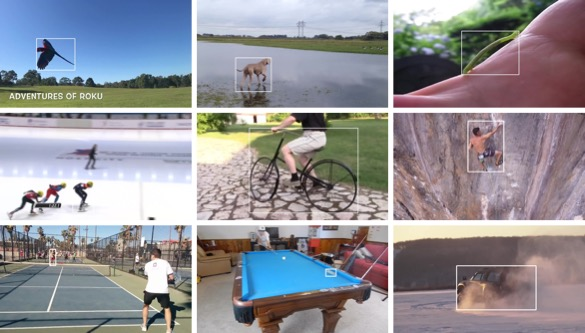
\includegraphics[width=\textwidth]{images/got10k}
%	\caption{
%		VOT
%		\textRL{لأغراض}
%		got10k \cite{got10k}
%		\textRL{عينات من مجموعة معطيات التدريب}
%	}	
%\end{figure}
%\selectlanguage{arabic}
أو
 عدة أهداف
\textLR{MOT}
%\selectlanguage{english}
%\begin{figure}[!h]
% 	\centering
% 	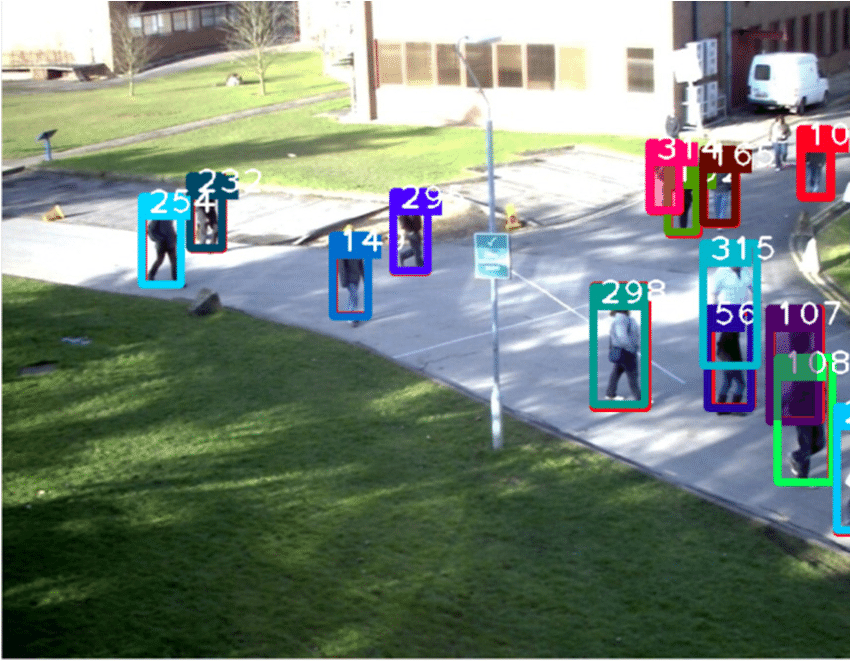
\includegraphics[width=\textwidth]{images/MOT15}
% 	\caption{
%		MOT
%		\textRL{لأغراض}
% 		\cite{Mot15}
% 		Mot15
% 		\textRL{ مثال عن مجموعة معطيات التدريب}
% 	}	
%\end{figure}
%\selectlanguage{arabic}
\item
ملاحقة سببية أو فورية
 \textLR{online tracker}،
غير سببية أو مؤجلة
 \textLR{offline tracker}:
\begin{itemize}
\item
خوارزميات ملاحقة غير سببية:
في بعض التطبيقات  كتحليل الفيديو مثلا، لا نحتاج إلى معرفة مكان الغرض  بشكل لحظي، عندها يمكن معالجة كامل صور  الفيديو دفعة واحدة، إذ يكون التركيز على دقة الملاحقة أكثر  من سرعة عملية المعالجة. وسميت بالملاحقات غير السببية لأن نتيجة الملاحقة لإطار معين يمكن أن تعتمد على الإطارات اللاحقة.
	
\item
خوارزميات ملاحقة سببية:
خرج الملاحقة من أجل الإطار الحالي يعتمد فقط على الإطارات السابقة، وهو الأكثر انتشاراً كون معظم تطبيقات الملاحقة تتطلب الحصول على النتيجة بشكل فوري.
	
\end{itemize}
\end{itemize}
نهتم في بحثنا بخوارزميات الملاحقة السببية، كاميرا واحدة، قصيرة المدى، و بالملاحقة بالزمن الحقيقي.
\section{أنواع خوارزميات الملاحقة التي تعتمد  التعلم العميق}
يمكن تصنيف ملاحقات التعلم العميق بحسب المرجع
\textLR{\cite{Marvasti}}
 كما يلي:
 \subsection{بنية الشبكة المستخدمة}
 إما أن تكون شبكات
 \textLR{Transformer,GAN,RNN,SNN,CNN}
 أو شبكة مصممة خصيصا لغرض الملاحقة
 \subsubsection{
 	الشبكات العصبونية التلافيفية
 \textLR{CNN Convolutional Neural Networks}}
استخدمت الشبكات التلافيفية في كثير من خوارزميات الملاحقة وذلك لقدرتها على إعطاء تمثيل للغرض بشكل أفضل من الشبكات الأخرى في حال وجود معطيات تدريب كافية،
لكنها غير ملائمة للتدريب أثناء الملاحقة
\textLR{online training}
بسبب التعقيد الحسابي الكبير.
مثل ملاحق 
 \textLR{MDNet \cite{MDNet}}.
 \begin{figure}[h!]
 	\centerline{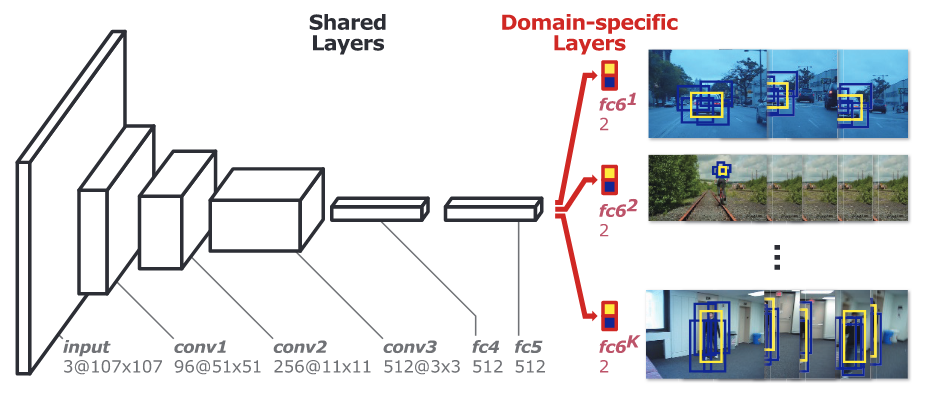
\includegraphics[width=\textwidth]{images/MDNet}}
 	\caption{\textRL{بنية الملاحق}
		\textLR{MDNet} 		 		
 		\textRL{الذي يستخدم شبكات تلافيفية}
 		\textLR{\cite{MDNet}}}	
 \end{figure}
\subsubsection{الشبكات التوأمية 
\textLR{SNN Siamese Neural Networks}}
سميت الشبكات التوأمية بذلك لأنها تتكون من شبكتين متطابقتين في البنية و الأوزان. في معظم تطبيقات الملاحقة يكون دخل الشبكة الأولى هو 
\textLR{template}
الغرض، أما دخل الشبكة الثانية فهو نافذة البحث. انتشر استخدام هذا النوع من الشبكات في خوارزمية الملاحقة بالزمن الحقيقي، لأنها ليست بحاجة إلى تعديل الأوزان أثناء الملاحقة، إذ يكفي تدريب الشبكة بشكل 
\textLR{offline}.
من الممكن أيضاً استخدام أي نوع من الشبكات ضمن الشبكة التوأمية مثل الشبكات التلافيفية كخوارزمية 
\textLR{GOTURN\cite{GOTURN}}
الموضحة في الشكل 
\ref{fig:GOTURN},
أو كمحول 
\textLR{Swin\cite{swintransformer}}
كما في 
\textLR{SwinTrack\cite{swinTrack}}
وهو النموذج الأساسي في بحثنا.
\begin{figure}[h!]
	\centerline{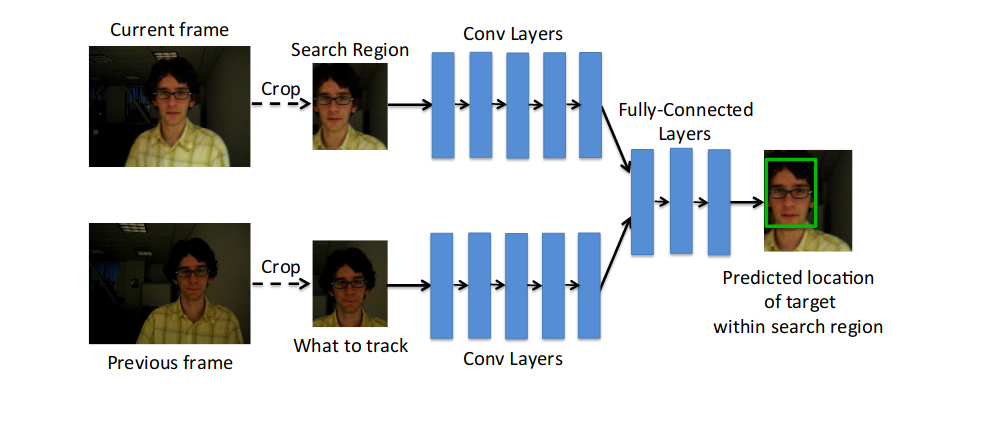
\includegraphics[width=\textwidth]{images/GOTURN}}
	\caption{
		\textRL{بنية الملاحق}
		\textLR{GOTURN}
		\textRL{الذي يستخدم شبكة توأمية مع تلافيفية}
		\textLR{\cite{GOTURN}}}	
	\label{fig:GOTURN}
\end{figure}
\subsubsection{الشبكات العصبونية العودية
\textLR{RNN Recurrent Neural Networks}}
بما أن الملاحقة لاتتعلق فقط بالمعلومات المكانية بل أيضاً بالمعلومات الزمانية، تم استخدام شبكات 
\textLR{RNN}
في مجال الملاحقة ولكن  بشكل محدود، نذكر منها خوارزمية 
\textLR{FPRNet}
\textLR{\cite{Ma18}}

\subsubsection{المحول 
\textLR{Transformer}}
لاقى نموذج المحول نجاحاً كبيراً في مجال معالجة اللغات الطبيعية 
\textLR{\cite{Vaswani17}}،
وبسبب هذا النجاح تم استخدامه في تطبيقات الرؤية الصنعية مثل كشف الأغراض كما في خوارزمية
\textLR{DETR\cite{DETR}}.
 وقد تم استغلاله لأغراض الملاحقة في العامين الأخيرين كما في خوارزميات 
\textLR{STARK\cite{Stark},
TrTr\cite{TrTr} ,
SwinTrack \cite{swinTrack}}.
\subsection{التدريب}
إما أن يكون التدريب 
\textLR{Online}
أو
\textLR{Offline}
 أو كلاهما معاً.
 الكثير من خوارزميات التعلم العميق تستفيد من خرج الشبكات المدربة مسبقاً على مهام مشابهة، والملاحقة مسألة مشابهة لكشف أو تصنيف الصور، لذلك نرى العديد من خوارزميات الملاحقات تستخدم شبكات مثل 
\textLR{ResNet\cite{ResNet},
VGG\cite{VGG}}
كـ
\textLR{backbone}
لاستخلاص السمات من الصور.


يمكن الاستفادة من بعض طبقات هذه الشبكات، أو تعديل بعض أو كل الأوزان بإجراء ضبط نهائي
\textLR{fine tuning}.
\subsubsection{
التدريب بشكل
\textLR{offline}}
معظم ملاحقات التعلم العميق تقوم بعملية التدريب بشكل
\textLR{offline}
وذلك بالاستفادة من مجموعات المعطيات الخاصة بالملاحقة مثل مجموعة المعطيات
\textLR{GOT-10k\cite{got10k},
	 LaSOT\cite{Lasot},
	 TrackingNet\cite{Trackingnet}}
وغيرها.
إذ أن التدريب بشكل  
\textLR{offline}
مناسب لتطبيقات الزمن الحقيقي لأن أوزان النموذج لاتحتاج إلى تعديل أثناء عملية الملاحقة، كما أن ذلك يقلل من انحياز النموذج نحو أغراض معينة 
\textLR{overfitting}
نتيجة التدريب بشكل 
\textLR{online}.
معظم الملاحقات الحديثة يتم تدريبها فقط بشكل 
\textLR{offline}
مثل
\textLR{
STARK\cite{Stark},
SiamRPN++\cite{SiamRPN++},
SwinTrack\cite{swinTrack}}
وغيرها الكثير.
\subsubsection{
التدريب بشكل 
\textLR{Online}
}
من المعروف أن تدريب نماذج التعلم العميق يحتاج زمن طويل وقدرة حسابية عالية، وفي حال عدم توفر عتاد صلب ملائم للتدريب من الممكن اللجوء إلى التدريب بشكل
\textLR{online}
لبعض النماذج، وذلك بتعديل بعض أو كامل أوزان النموذج.
نذكر منها خوارزمية 
\textLR{DeepTrack\cite{DeepTrack},SMART\cite{SMART}}.

\subsubsection{التدريب 
\textLR{online}
و 
\textLR{offline}
معاً}
يمكن جمع طريقتي التدريب السابقتين وذلك بتدريب النموذج بشكل
\textLR{offline}
في البداية
باستخدام مجموعات المعطيات الخاصة بالملاحقة، وبعد ذلك يتم تعديل كامل أو بعض أوزان النموذج أثناء عملية الملاحقة. وذلك كما في خوارزميات 
\textLR{ATOM\cite{ATOM},
	 MDNET\cite{MDNet},
	 DiMP\cite{DIMP},
	 PrDiMP\cite{prDIMP}}.
\subsubsection{}
و كغيرها من نماذج تعلم الآلة فإن خوارزميات الملاحقة التي تعتمد تقنيات التعلم العميق تستخدم تعزيز المعطيات
\textLR{data  augmentation}
 لتقليل الـ
\textLR{ overfitting}،
 وهي طريقة لزيادة حجم مجموعة المعطيات باستخدام بعض التقنيات كاستخدام تحويلات إما في الفضاء الهندسي أو اللوني أو غيرها.
\subsection{غرض الشبكة}
إما أن يكون غرض الشبكة التصنيف 
\textLR{classification}
 أو الـ 
\textLR{regression}
 أو كلاهما معاً.

\subsubsection{التصنيف}
تستخدم الكثير من  الملاحقات أساليب الخوارزميات الأخرى المشابهة لها في  المهام ككشف أو تصنيف الأغراض في الصور وغيرها، ومن هذه الأساليب هي توليد العديد من المناطق المرشَّحة تدعى بـ
\textLR{candidates}
أو بـ
\textLR{proposal bounding boxes}
 المستخلصة من نافذة البحث، ويكون هدف الشبكة هو تصنيف هذه المناطق إما كغرض أو كخلفية. وبالتالي يدرب النموذج وفق هذا المعيار وتستخدم العديد من توابع الخسارة لهذا الغرض مثل 
\textLR{cross-entropy CE,
	focal loss FL\cite{FocalLoss}،
	varifocal loss VL\cite{varifocal}}،
وغيرها، كملاحقات 
\textLR{SiamFC\cite{SiamFC} , DeepTrack\cite{DeepTrack}}.
\subsubsection{
\textLR{Regression}
}
غرض الشبكة في هذه الحالة هو تحديد مكان وأبعاد المستطيل المحيط للغرض بشكل مباشر باستخدام توابع خطأ تعتمد على
\textLR{L1}
 أو
\textLR{L2}،
كما في 
\textLR{GOTURN\cite{GOTURN}}.

\subsubsection{التصنيف والـ
\textLR{regression}
معاً}
 العديد من الملاحقات  قد استخدمت كلتا الطريقتين للتنبؤ بمكان الهدف، إذ يتم توليد العديد من المناطق المرشحة وتحديد المنطقة الأكثر شبهاً بالغرض من خلال شبكة تصنيف، وتحديد أبعاد المستطيل المحيط و زيادة دقة التنبؤ بموقع الغرض من خلال شبكة 
\textLR{regression}،
كما في 
\textLR{MDNet\cite{MDNet}, SwinTrack\cite{swinTrack}, DiMP\cite{DIMP}, SiamRPN++\cite{SiamRPN++}} 
وغيرها.
\subsection{خرج الشبكة}
تبعاً لغرض الشبكة فإن الخرج يمكن أن يكون
\begin{itemize}
	\item خريطة الاستجابة: او ما يدعى بـ 
	\textLR{Confidence}
أو
	\textLR{Response Map}
وهي عبارة عن مصفوفة من القيم ضمن المجال
	$[0,1]$،
وكل قيمة تعبر عن احتمالية وجود الغرض  في الموقع المقابل لها	كما في 
	\textLR{SiamFC\cite{SiamFC}, ATOM\cite{ATOM}, DiMP\cite{DIMP}, SMART\cite{SMART}, PrDiMP\cite{prDIMP}}.
	\item 
	المستطيل المحيط بالغرض: ويمكن أن يعبر عنه بإحداثيات زاويتي المستطيل المتقابلتين، أو بإحداثيات المركز مع أبعاد المستطيل،
	كما في 
	\textLR{GOTURN\cite{GOTURN}, SiamRPN++\cite{SiamRPN++}}
	\item 
	نتيجة التشابه
		 \textLR{similarity score}
		 مثل
		 \textLR{MDNet\cite{MDNet}, DeepTrack \cite{DeepTrack}, SiamRPN++ \cite{SiamRPN++}}
	\item 
	قناع التجزئة
	\textLR{Segmentation Mask}
	مثل خوارزمية 
	\textLR{SiamAttn \cite{SiamAtt}}.
\end{itemize}
هذا فيما يخص أنواع خوارزميات الملاحقة، في الفقرة التالية سنشرح عن نموذج المحول، وعن النماذج السابقة له وكيفية تطور بنيته، وسنشرح عن تابع الانتباه 
\section{النماذج السابقة للمحول}
صمم نموذج المحول
\textLR{\cite{Vaswani17}}
ليكون إحدى نماذج
\textLR{seq2seq}،
وهي نماذج يكون كل من دخلها وخرجها عبارة عن سلاسل من العناصر. من الممكن أن تكون السلسلة أي نوع من المعلومات ككلمات، صور، محارف أو غيرها
\textLR{\cite{web:visualize}}.
\newline
معظم تطبيقات نماذج
\textLR{seq2seq}
 كانت في مجال معالجة اللغات الطبيعية
\textLR{Natural Language Processing NLP}
 أي يكون الدخل عبارة عن سلسلة من كلمات.
\begin{figure}[h!]
\centerline{
	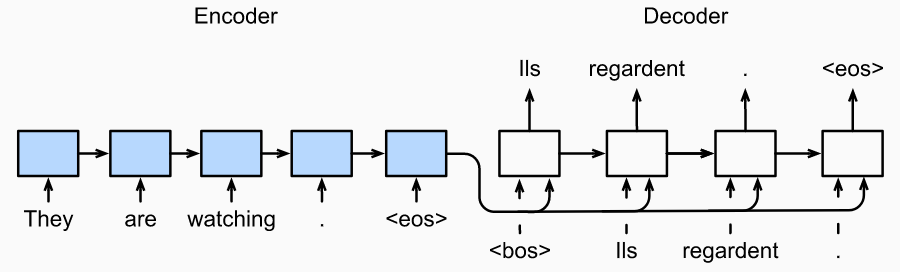
\includegraphics[width=\textwidth]{images/RNN.png}}
\caption{نموذج
\textLR{seq2seq}
مع بنية
\textLR{encoder-decoder}
\textLR{\cite{d2l_rnn}}
}
\label{fig:RNN1}	
\end{figure}
%قبل استخدام نموذج المحول
كانت البنية الأساسية لنماذج
\textLR{seq2seq}
هي الشبكات العصبونية العودية
\textLR{recurrent neural networks RNN}.
ولفهم تطور بنية المحول يجب أن نفهم البنية العامة للشبكات العودية وهو ما سنذكره في الفقرة القادمة.
\newline
\subsection{الشبكات العصبونية العودية
\textLR{RNN}
}
تُستخدم
\textLR{RNN}
 بشكل رئيسي للتعرف على الأنماط في المعطيات التسلسلية، كالنصوص، الفيديوهات أو أي متسلسلة زمنية. وما يميزها
 عن الشبكات العصبونية التقليدية
\textLR{MLP Multilayer perceptron}
 هو كيفية مرور المعلومات من خلالها
\textLR{\cite{RNN-gentleIntro}}.

\begin{figure}[H]
	\centerline{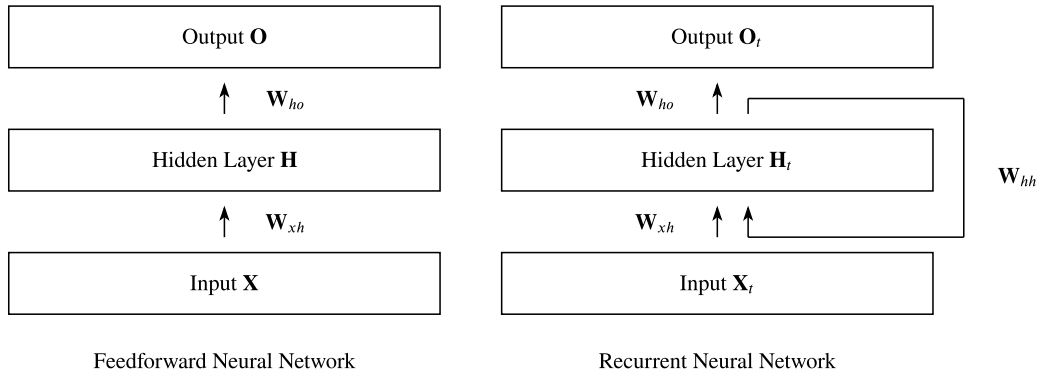
\includegraphics[width=\textwidth]{images/RNN_gentle_introduction.png}}
	\caption{
	\begin{footnotesize}
			الفرق بين مرور المعلومات بين الشبكات العودية - اليمين، والشبكات التقليدية - اليسار
\textLR{\cite{RNN-gentleIntro}}
	\end{footnotesize}
		}
	\label{fig:RNN2}
\end{figure}
يوضح الشكل
\ref{fig:RNN2}
 الاختلاف بين
\textLR{MLP}
 و
\textLR{RNN}،
 حيث تمرر شبكات 
\textLR{MLP}
المعلومات بدون وجود أي حلقات على العكس من شبكات
\textLR{RNN}.
حيث يحسب الخرج في شبكات
\textLR{MLP}
 كما في المعادلات
\ref{eq:mlp}
\begin{equation}
	\begin{split}
	& H = \phi_h (XW_{xh} + b_h)\\
	& O = \phi_o (HW_{ho} + b_o)\\
	\end{split}
	\label{eq:mlp}
\end{equation}
حيث $H$ خرج الطبقة المخفية، 
$\phi_h$
تابع تفعيل الطبقة المخفية،
$O$
الخرج النهائي،
$\phi_o$
تابع تغعيل طبقة الخرج، 
$W,b$
مصفوفات الأوزان وأشعة الانحياز.
\newline
أما في 
\textLR{RNN}
فمعادلة الخرج في كل خطوة زمنية
$t$
تحسب من خلال المعادلات 
\ref{eq:RNN}
\begin{equation}
\begin{split}
	&H_t = \phi_h(X_t W_{xh} + H_{t-1} W_{hh} + b_h)\\
	& O_t = \phi_o (H_t W_{ho} + b_o)\\
\end{split}
\label{eq:RNN}
\end{equation}
حيث
$H_t$
يدعى بالحالة المخفية
\textLR{hidden state}
في اللحظة
$t$.
\newline
نلاحظ أنه في كل خطوة زمنية لحساب الخرج نحتاج إلى الدخل
$X_t$
وإلى الحالة المخفية في الخطوة الزمنية السابقة كما هو موضح في الشكل 
\ref{fig:RNN3}،
والذي يبين مخارج ومداخل
\textLR{RNN}
بعد نشر الشبكة من أجل كل خطوة زمنية.
\begin{figure}[h!]
	\centerline{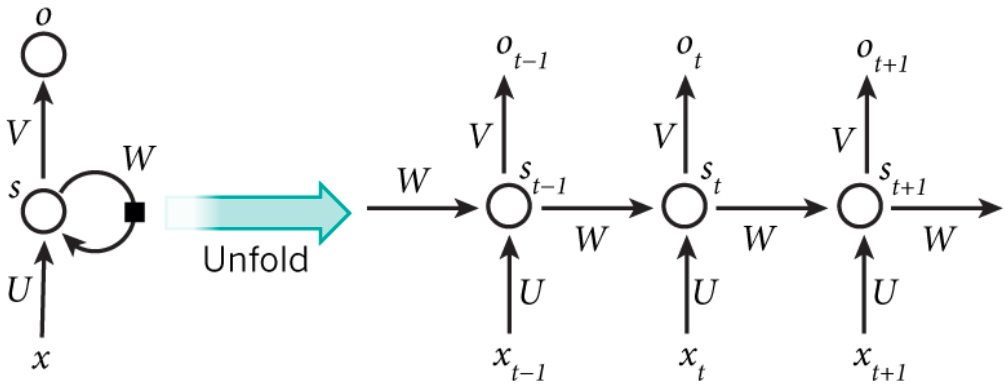
\includegraphics[width=\textwidth]{images/RNN_unfold}}
	\caption{
		نشر الشبكة العصبونية العودية
		\textLR{RNN}
		من أجل عدة لحظات زمنية
		\textLR{\cite{RNN-unfold}}}
	\label{fig:RNN3}
\end{figure}
%نلاحظ أيضا أنه لحساب الخرج في لحظة زمنية
%$t$
%نحتاج إلى دخل السلسلة في هذه اللحظة
%$X_t$
%وإلى الحالة المخفية في اللحظة السابقة
%$H_{t-1}$
%أو
%$s_{t-1}$
%كما هو موضح في الشكل
%\ref{fig:RNN3}
%والمعادلات
%\ref{eq:RNN}.
\newline
\subsubsection{مشكلات 
\textLR{RNN}}
إحدى سلبيات شبكات
\textLR{RNN}
 هي معالجة العناصر بشكل تسلسلي، فكما رأينا في الفقرة السابقة فإن الخرج في كل خطوة زمنية يحتاج إلى معالجة المداخل السابقة بشكل تسلسلي و هذا مايجعل زمن التدريب طويلاً، وبسبب بنية الشبكة تصبح المعالجة بشكل تفرعي أمراً صعباً أو حتى مستحيل
\textLR{\cite{TransformerCV}}.
المشكلة الثانية هي تلاشي المشتقات
\textLR{vanishing gradient}
وهو ما يزيد من صعوبة التدريب وبخاصة في حالة السلاسل الطويلة، إحدى أشهر الحلول لتقليل أثر هذه المشكلة هي باستخدام
\textLR{Long Short-Term Memory LSTM}.
من الممكن أن تختلف أبعاد سلسلتي الدخل والخرج ولحل هذا الاختلاف في الطول يمكن استخدام شبكتين عوديتين منفصلتين الأولى نسميها الـ
\textLR{encoder}
المرمز والثانية الـ
\textLR{decoder}
مفكك ترميز.
\subsection{
بنية المرمز ومفكك الترميز
}
يعالج المرمز كل عنصر من عناصر سلسلة الدخل ويستخرج المعلومات ويضعها في شعاع يسمى شعاع السياق
\textLR{context vector}،
بعد انتهاء المرمز من معالجة كامل عناصر الدخل يرسل شعاع السياق إلى مفكك الترميز
%\textLR{decoder}
 ليقوم بتوليد سلسلة الخرج بشكل تتابعي كما في الشكل
\ref{fig:RNN1}.
\newline
المشكلة الأساسية في هذه النماذج هي كيفية توليد شعاع السياق ليعبر بأفضل طريقة ممكنة عن معلومات سلسلة الدخل. فإذا كان شعاع السياق هو الحالة المخفية لآخر خطوة زمنية في سلسلة الدخل عندها لن يعبر بشكل فعال عن بدايات السلسلة وخصوصاً في حالة سلسلة الدخل الطويلة
\textLR{\cite{IllustratedAttention}}.
عندها يمكن أن يكون شعاع السياق عبارة عن كامل الحالات المخفية لكل خطوة زمنية في سلسلة الدخل، أو أن ينتج عن تعديل هذه الحالات المخفية بتطبيق تابع معين، ومن هنا ظهرت فكرة الانتباه 
\textLR{attention}،
وذلك بالتركيز فقط على الأجزاء المهمة وجعل الأجزاء غير المهمة أقل تأثيراً
\textLR{\cite{TransformerCV}}.
بما أن المشكلة الأساسية هي كيفية توليد شعاع السياق كان هناك الكثير من الأبحاث لتحسين تمثيل هذا الشعاع من أبرزها
\textLR{\cite{Bahdanau2016},\cite{Luong2015}}.
إذ كانت هذه الأعمال بدايات فكرة الانتباه، والذي أظهر نتائج جيدة ومبشرة في تطبيقات ترجمة الآلة، وخاصة في حالة الأبعاد الكبيرة لسلاسل الدخل
\textLR{\cite{IllustratedAttention}}.

\section{المحول \label{section:transformer}}
ظهر نموذج المحول
\textLR{Transformer\cite{Vaswani17}}
في عام $2017$ ولأول مرة تم اختبار نموذج يعتمد بشكل كامل على توابع الانتباه ويستغني عن
\textLR{RNN}،
 مما جنب نموذج المحول العديد من مشاكل هذا النوع من الشبكات والتي أهمها عدم القدرة على المعالجة التفرعية لعناصر الدخل، إذ أن أحد ميزات المحول هي قابلية معالجة العمليات الحسابية بشكل تفرعي كما سنرى لاحقاً وهذا ما يسرع عملية التدريب و الـ 
\textLR{inference}
في حال وجود
\textLR{GPU}.
\subsection{بنية المحول}
\begin{table}[h!]
	\centering
	\begin{tabular}{c c} 
		\hline
		\textLR{sympol} & \textLR{meaning} \\ [0.5ex] 
		\hline\hline
		$d$ & \textRL{بعد النموذج}  \\ 
		$h$ &  \textLR{MHA} \textRL{عدد الرؤوس في}\\
		$L$ & \textLR{tokens} \textRL{عدد عناصر سلسلة الدخل، أو عدد الـ}\\
		$X \in \mathds{R}^{L \mathsf{x}d}$&\textRL{دخل المرمز}\\
		$W^k \in \mathds{R}^{d \mathsf{x} d_x}$&\textLR{key}\textRL{مصفوفة الأوزان لشعاع الـ }\\
		$W^q \in \mathds{R}^{d \mathsf{x} d_x}$&\textLR{query}\textRL{مصفوفة الأوزان لشعاع الـ }\\
		$W^v \in \mathds{R}^{d \mathsf{x} d_v}$&\textLR{value}\textRL{مصفوفة الأوزان لشعاع الـ }\\
		$W^k_i,W^q_i \in \mathds{R}^{d\mathsf{x}d_k/h};W^v_i\in \mathds{R}^{d\mathsf{x}d_v/h}$&\textRL{مصفوفات الأوزان لكل  رأس}\\
		$W^o \in \mathds{R}^{d_v \mathsf{x}d}$&\textRL{مصفوفة الأوزان لشعاع الخرج }\\
		$Q = XW^q \mathds{R}^{L \mathsf{x}d_k}$&\textLR{query}\\
		$K = XW^k \mathds{R}^{L \mathsf{x}d_k}$&\textLR{key}\\
		$V = XW^v \mathds{R}^{L \mathsf{x}d_v}$&\textLR{value}\\
		\hline
	\end{tabular}
	\caption{\textRL{الرموز المستخدمة في شرح بنية المحول مع أبعاد المصفوفات}}
	\label{table:transformer_sympols}
\end{table}          
إن التطبيق الأساسي لنموذج المحول الأصلي
\textLR{\cite{Vaswani17}}
هو ترجمة الجمل من اللغة الإنكليزية إلى لغات أخرى، إذ أن دخل النموذج سلسلة من الكلمات (عدة جمل)، كل كلمة يتم التعبير عنها بشعاع من الأرقام ندعوه بالـ
\textLR{token}،
فيكون دخل المرمز هو عبارة عن مصفوفة أشعة
$X \in \mathds{R}^{L \mathsf{x}d}$.
\newline
لتمييز مكان كل عنصر من السلسلة  يتم إضافة قيم للترميز المكاني
\textLR{positional encoding PE}.
خرج كل طبقة من طبقات المرمز وطبقات مفكك الترميز
هو مصفوفة أشعة بأبعاد
$L \mathsf{x} d$.
كما يوضح الشكل
\ref{fig:Transformer}
يتكون كل من المرمز و مفكك الترميز
 من عدة كتل متسلسلة ومتطابقة في البنية.
\subsection{المرمز}
بداخل كل كتلة مرمز كتلتان أساسيتان كما في الشكل
\ref{fig:enc_dec}
 الأولى لحساب الانتباه الذاتي متعدد الرؤوس 
\textLR{Multi-Head Self Attention MHA},
مهمة هذا التابع هو تعديل تمثيل عناصر سلسلة الدخل بحسب السياق.
والكتلة الثانية هي شبكة عصبونية
\textLR{FFN}
تتكون من طبقتين مع تابع تفعيل 
\textLR{ReLU}
بحسب المعادلة
\ref{eq:MLP}.
\begin{equation}
FFN(x) = max(0,xW_1+b_1)W_2+b_2
\label{eq:MLP}
\end{equation}
تطبق هذه الشبكة على كل
\textLR{token}
أو عنصر دخل بشكل منفصل ومتطابق، وهذا مانسميه
\textLR{position-wise}
كما في الشكل
\ref{fig:positionWise}،
مما يجعل المحول قادر على إجراء الحسابات بشكل تفرعي.
من أجل كل من الكتلتين السابقتين يتم تطبيق
\textLR{residual connection \cite{residual}}،
 متبوعة بـ
\textLR{layer normalization\cite{LN}}.
\newline
%$\text{\textLR{LayerNorm}}(x+\text{\textLR{Sublayer}}(x))$
%حيث
%\textLR{sublayer}
%هي تابع الانتباه أو الشبكة العصبونية الأمامية.
\begin{figure}[H]
	\centerline{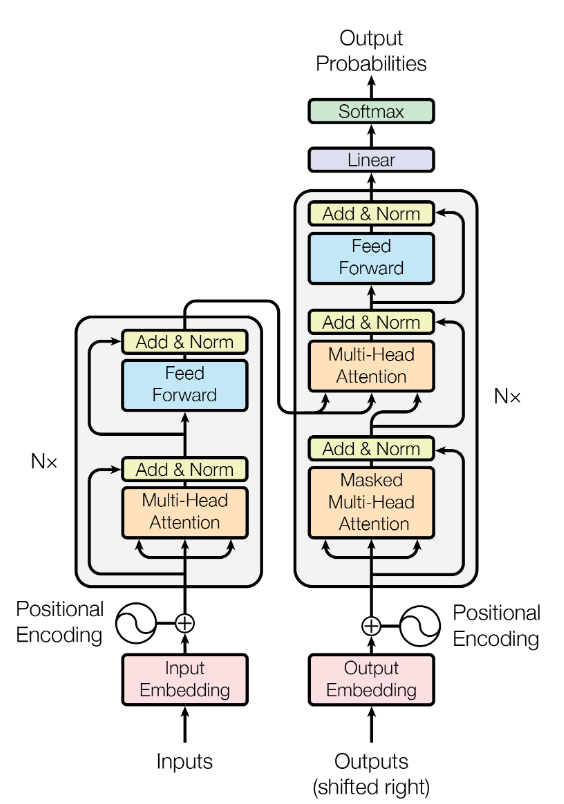
\includegraphics[scale=0.5]{images/Transformer}}
	\caption{\textRL{البنية الأساسية للمحول}
	\textLR{\cite{Vaswani17}}}
	\label{fig:Transformer}
\end{figure}

\begin{figure}[h!]
	\centerline{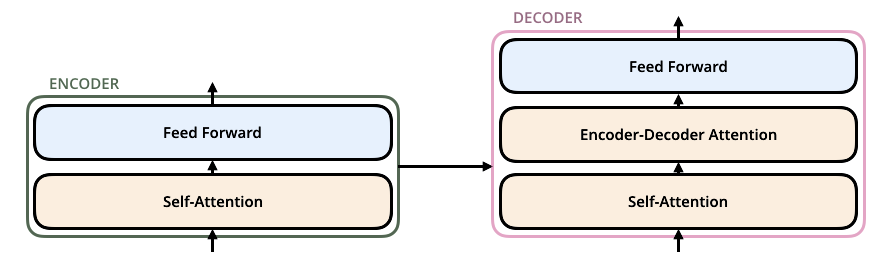
\includegraphics[scale=0.3]{images/encoder_decoder_illustrated_transformer}}
	\caption{البنية الأساسية للمرمز و مفكك الترميز
		داخل المحول
		\textLR{\cite{illustratedTransformer}}}
	\label{fig:enc_dec}
\end{figure}

\begin{figure}[h!]
	\centerline{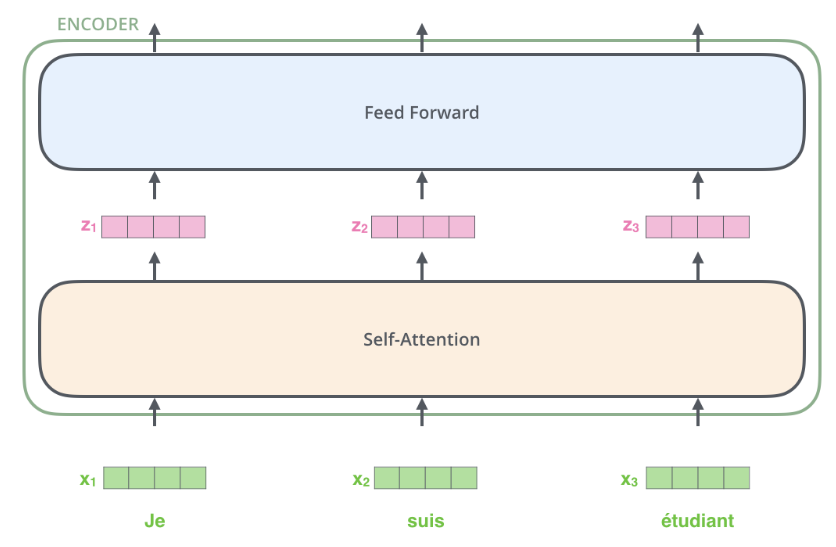
\includegraphics[scale=0.3]{images/position_wise_illustrated_transformer}}
	\caption{\textRL{تطبيق التوابع داخل المحول لكل عنصر دخل بشكل تفرعي}
	\textLR{\cite{illustratedTransformer}}}
	\label{fig:positionWise}
\end{figure}
 
\subsection{مفكك الترميز}
يوضح الشكلان
\ref{fig:Transformer}،\ref{fig:enc_dec}
بنية مفكك الترميز،
وكما في المرمز فإنه يتكون بالإضافة إلى كتلتي الانتباه الذاتي والشبكة الأمامية فإنه أيضاً يحتوي على كتلة إضافية وهي الانتباه التقاطعي متعدد الرؤوس.
%\ref{MCHA}
%دخل هذا التابع هو دخل مفكك الترميز بعد إضافة الترميز المكاني، بحيث يكون %دخل مفكك الترميز  هو خرج آخر طبقة في المرمز.
في خوارزمية المحول الأساسية
\textLR{\cite{Vaswani17}}
يكون دخل مفكك الترميز  هو خرج آخر طبقة في المرمز.
\subsection{ترميز المعلومات المكانية
\textLR{positional encoding\label{PE}}}
كما ذكرنا سابقاً فإن معظم نماذج
\textLR{seq2seq}
قبل ظهور نموذج المحول
\textLR{\cite{Vaswani17}}
كانت تستخدم الشبكات العودية
\textLR{RNN}
مع 
\textLR{LSTM}،
وهذا النوع من الشبكات يحافظ على المعلومات المكانية النسبية لعناصر سلسلة الدخل،  لكن الاستغناء عن شبكات 
\textLR{RNN}
والاستعانة فقط بتوابع الانتباه لمعالجة السلاسل يفقد المعلومات المكانية.
\newline
لمعالجة هذه المشكلة كان من اللازم إدخال المعلومات المكانية للسلسلة بشكل ما، هنا تم طرح طريقة ترميز الموقع لإضافة المعلومات المكانية لكل عنصر من عناصر السلسلة وذلك بإضافة قيم مستخرجة من توابع بترددات مختلفة كما في المعادلات 
\ref{eq:PE}
\textLR{\cite{Vaswani17}}.
\begin{equation}
\begin{split}
	&PE_{(pos,2i)} = sin(pos/1000^{2i/d_{model}})\\
	&PE_{(pos,2i+1)} = cos(pos/1000^{2i/d_{model}})\\
\end{split}
\label{eq:PE}
\end{equation}
حيث 
\textLR{pos}
موقع عنصر الدخل من السلسلة، و
$i$
هو البعد 
\textLR{dimension}.
ويتم إضافة قيم هذه التوابع إلى دخل كل من المرمز ومفكك الترميز.
\newline
اختبرت العديد من الأبحاث طرق الترميز المكاني، فأبسط الأشكال هي إسناد رقم طبيعي أو حقيقي مميز أو عدد ضمن المجال
$[0,1]$
 إلى كل عنصر من عناصر السلسلة
\textLR{\cite{web:PE}}.
\newline
لكن هذه الطرق البسيطة لم تحسن النتائج لأنها لم تستطع أن تجعل النموذج يلتقط معلومات المواقع بين العناصر.
هنا اقترح البحث 
\textLR{\cite{Vaswani17}}
أن يكون ترميز الموقع تابع جيبي كما في المعادلات 
\ref{eq:PE}،
إذ يمكن اعتبار  سلسلة الدخل سلسلة زمنية وكل عنصر هو خرج السلسلة عند خطوة زمنية معينة
\textLR{\cite{web:PE}}،
هذه الطريقة في التفكير ساعدت النموذج على كشف معلومات الموقع النسبية بين العناصر.
 
في الملاحق المستخدم في بحثنا
\textLR{SwinTrack\cite{swinTrack}\ref{section:swintrack}}
تم استخدام 
\textLR{untied PE \cite{untiedPE}}
مع بارامترات قابلة للتدريب.
\subsection{تابع الانتباه\label{att}}
كما ذكرنا في الفقرات السابقة فإن تابع الانتباه هو الجزء الأساسي في نموذج المحول، لذلك وجب شرحه بشيء من التفصيل في الفقرة الحالية، إذ سنشرح عن التابع بشكل عام وعن مفهوم الانتباه، ثم سنشرح عن طريقة استخدامه في نموذج المحول.
\subsubsection{الفكرة العامة لتابع الانتباه الذاتي 
\textLR{self-attention}
\label{section:att_example}
}
لتبسيط شرح مفهوم تابع الانتباه الذاتي سنقوم بالاستعانة بمثال بسيط عن الترجمة، إذ يمكن إسقاط هذا المثال على مجالات أخرى كالرؤية الحاسوبية، وذلك باعتبار $"$الكلمة$"$ مقابلة لـ $"$البكسل$"$ أو $"$مجموعة من البكسلات$"$.
\newline
لنأخذ كمثال جملة 
\textLR{Bank of a river}.
\newline
بداية نحول كل كلمة إلى تمثيل رقمي ندعوه بالـ
\textLR{token}
عبر
\textLR{word embedding}.
هناك العديد من الخوارزميات المدربة مسبقاً لهذا الغرض، بحيث تكون الكلمات المتشابهة بالمعنى $"$متشابهة$"$ أيضاً بالتمثيل الرقمي (أي أن الجداء السلمي لها قيمة قريبة من الواحد). عندها يمكن تمثيل الجملة السابقة كما يلي:
\newline
\textLR{Bank of a river}
\newline
$[word_1, word_2, word_3, word_4]$
\newline
بعد تحويل الـ
\textLR{embedding}
\newline
$X = [x_1,x_2,x_3,x_4]$
\newline
كما ذكرنا سابقاً هدف الانتباه هو تعديل شعاع الـ
\textLR{embedding}
ليناسب السياق. سنشرح فيما يلي كيف يتم ذلك.
\newline
أولاً نحسب التشابه بين كل كلمة في الجملة مع كل كلمات الجملة وذلك عن طريق الجداء السلمي 
\textLR{dot-product}
كما في المعادلات
\ref{eq:att_dot_product}.
\begin{equation}
\begin{split}
&s_{11} = x_1.x_1\\
&s_{12} = x_1.x_2\\
&\text{...}\\
&s_{ij} = x_i.x_j\\
\end{split}
\label{eq:att_dot_product}
\end{equation}
نطبق
\textLR{softmax}
لجعل قيم التشابه ضمن المجال
$[0,1]$
بحيث يكون التشابه بين الكلمة $i$ وكامل الجملة كما في المعادلة 
\ref{eq:att_softmax}.
\begin{equation}
score_{i1},score_{i2},... = softmax(s_{i1},s_{i2},..)
\label{eq:att_softmax}
\end{equation}
من خلال استخدام تابع الانتباه يتم تعديل تمثيل الكلمة $x_i$  بحسب التشابه بينها وبين كلمات الجملة أي بحسب قيم الـ $score_{ij}$، فيكون التمثيل المعدل كما في المعادلة 
\ref{eq:att_fin}>
\begin{equation}
x_{i_{new}} = score_{i1}*x_1+score_{i2}*x_2+...
\label{eq:att_fin}
\end{equation}
وبهذه الطريقة يتغير تمثيل كل كلمة بحسب السياق الكامل للجملة. 
\newline
يستخدم نموذج المحول تابع انتباه مع أشعة تسمى بـ
\textLR{Query ,Keys,Values}،
هذه التسمية مستوحاة من أنظمة الاسترجاع
\textLR{retrieval systems}.
بشكل عام يكون لتابع الانتباه  شعاعا دخل
$X_1,X_2$،
يولد
$X_2$
الـ
\textLR{Query}،
ويولد
$X_1$
كل من الـ
\textLR{Key,Value}،
وذلك باستخدام مصفوفات
$W_q,W_v,W_k$
عناصرها أوزان قابلة للتدريب كما في المعادلات 
\ref{eq:att_mat}.
\begin{equation}
\begin{split}
&Q = X_2 W_q\\
&K = X_1 W_k\\
&V = X_1 W_v\\
\end{split}
\label{eq:att_mat}
\end{equation}
بالنسبة لتابع الانتباه الذاتي يكون
$X_1 = X_2$.
أما في الانتباه التقاطعي الذي سنذكره لاحقاً في الفقرة
\ref{section:attention}
فإن
$X_1$
مصدرها خرج المرمز، أما
$X_2$
فمصدرها مفكك الترميز.
\subsubsection{الانتباه\label{section:attention}}
 هناك نوعان من الانتباه في نموذج المحول، الانتباه الذاتي
\textLR{self-attention}،
والانتباه التقاطعي
\textLR{cross-attention}.
بالنسبة لتابع الانتباه الذاتي له ثلاث مداخل وهي
\textLR{Q query,K key,V value}،
هذه المصفوفات ناتجة عن ضرب مصفوفة الدخل
$X$
في كل طبقة مرمز بمصفوفات
$W_q,W_v,W_k$
 بالتسلسل كما في المعادلات
\ref{eq:att_mat}،
وعناصر هذه المصفوفات هي أوزان تحدد قيمها أثناء التدريب.
\newline
يمكن أيضاً أن نعبر عن تابع الانتباه باستخدام مصفوفات
$Q,K,V$
بالمعادلة
\ref{eq:att}
\textLR{\cite{Vaswani17}}
وكما يوضحه الشكل 
\ref{fig:att_dot_prod}.
\begin{equation}
\begin{split}
Attention(Q,K,V) = softmax(\frac{QK^T}{\sqrt{d_k}})V
\label{eq:att}
\end{split}
\end{equation}
\begin{figure}[h!]
\centerline{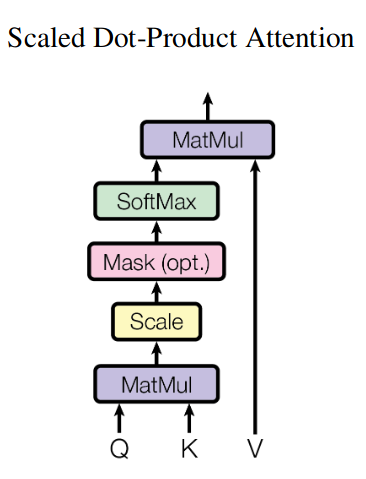
\includegraphics[scale=0.4]{images/att_dot_prod.png}}
\caption{\textRL{حساب تابع الانتباه عن طريق الجداء السلمي المقيس}
\textLR{\cite{Vaswani17}}}
\label{fig:att_dot_prod}
\end{figure}
إذ نلاحظ أن تابع الانتباه يتكون من مرحلتين، المرحلة الأولى هي حساب الـ
\textLR{score}
\begin{equation}
score(Q,K) = softmax(\frac{QK^T}{\sqrt{d_k}})
\end{equation}
والمرحلة الثانية هي تعديل مصفوفة القيم
$V$
بحسب قيم الـ
\textLR{score}.
إن دخل وخرج تابع الانتباه في المعادلة
\ref{eq:att}
هو عبارة عن مصفوفات.
\newline
ولفهم كيف يؤثر هذا التابع على كل شعاع
\textLR{token}
من أشعة الدخل،
نحسب الانتباه الذاتي للشعاع
$x_i$
من مصفوفة الدخل 
$X$.
بداية نحسب كل من قيمة
$k_i,q_i,v_i$
بحسب المعادلات
\ref{eq:att_mat_i}.
\begin{equation}
\begin{split}
&k_i = x_i W_k\\
&q_i = x_i W_q\\
&v_i = x_i W_v\\
\end{split}
\label{eq:att_mat_i}
\end{equation}
نحسب الجداء السلمي بين
$q_i$
وبين كل عنصر من عناصر المصفوفة
$K$ 
كما في المعادلات
\ref{eq:att_mat_i2}.
كما نعلم بأن الجداء السلمي يقيس مدى التشابه بين الشعاع
$q_i$
وبين أشعة المصفوفة
$K$.
ومن ثم نقيّس هذه القيم بتقسيمها على
$\sqrt{d_k}$،
حيث 
$d_k$
هو بعد النموذج 
%كما في الجدول 
%\ref{table:transformer_sympols}
أي بعد شعاع الدخل.
وقد وجد أن التقسيم على هذه القيمة جعل المشتق أكثر استقراراً
\textLR{\cite{illustratedTransformer}}.
ومن ثم بحساب الـ
\textLR{softmax}
والذي يضمن أن تكون القيم مقيسة بين
$[0,1]$،
خرج الـ
\textLR{softmax}
ندعوه بالـ
\textLR{score}.
 وقيم الـ
\textLR{score}
تحدد العناصر التي يجب التركيز عليها أثناء حساب خرج المرمز.
\begin{equation}
	\begin{split}
	&s_{11} = q_1.k_1\\
	&s_{12} = q_1.k_2\\
	&...\\
	&s_{1d} = q_1.k_d\\
	&score =score_1,score_2,..= softmax(\frac{s_{11}}{\sqrt{d_k}},\frac{s_{12}}{\sqrt{d_k}},...)\\
	\end{split}
	\label{eq:att_mat_i2}
\end{equation}
يوضح الشكل 
\ref{fig:att_score}
المرحلة الأولى من تابع الانتباه
\begin{figure}[H]
	\centerline{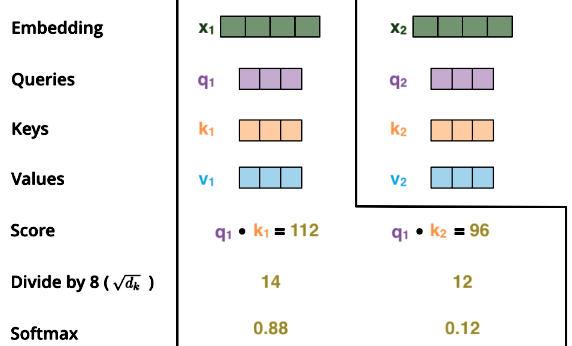
\includegraphics[scale=0.4]{images/att_score}}
	\caption{\textRL{ مثال رقمي عن حساب الـ}
		\textLR{score}
		\textRL{لتابع الانتباه عن طريق الجداء السلمي}
		\textLR{\cite{IllustratedAttention}}}
	\label{fig:att_score}
\end{figure}
المرحلة الثانية هي بحساب الخرج النهائي لتابع الانتباه
$z_1$
 وذلك بالتركيز على قيم 
$V$
بحسب التشابه بين 
$q,K$
كما في المعادلة 
\ref{eq:att_mat_fin}،
وكما يوضحه الشكل 
\ref{fig:att_output}،
وبالمثل نحسب
$z_2,z_3,...$.
\begin{equation}
z_1 = score_1.v_1 + score_2.v_2+....
\label{eq:att_mat_fin}
\end{equation}
\begin{figure}[H]
	\centerline{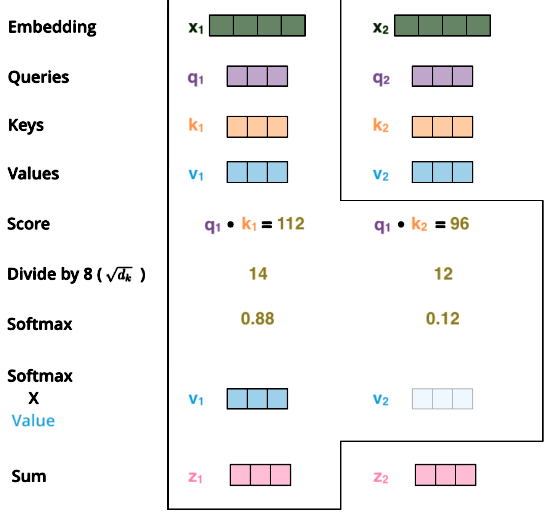
\includegraphics[scale=0.4]{images/attention_output.png}}
	\caption{\textRL{شكل توضيحي لحساب الانتباه من أجل كل عنصر دخل}
		\textLR{\cite{illustratedTransformer}}}
	\label{fig:att_output}
\end{figure}
%ونلاحظ من حساب الخرج أننا نقوم بالتركيز على قيم
%$V$
%بحسب التشابه بين 
%$q,K$.
%وبالمثل نحسب
%$z_2,z_3,...$.
%ويمكننا أن نحول الحساب إلى جداء مصفوفات مباشرة كما في معادلة حساب الانتباه 
%\ref{eq:att}.
\subsubsection{ الانتباه المتعدد الرؤوس
\textLR{Multi-head attention MHA}
}
إحدى الإضافات المهمة في نموذج المحول هي استخدام الانتباه المتعدد الرؤوس. وفيها يحسب الانتباه عدة مرات بحسب عدد الرؤوس
$h$
بشكل تفرعي، كما يوضحه الشكل
\ref{fig:MHA}
\begin{figure}[h!]
	\centerline{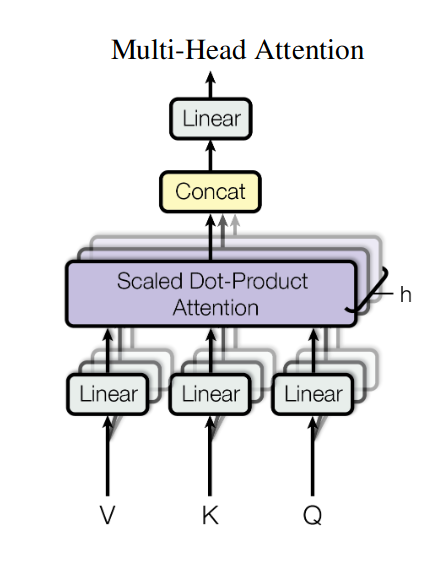
\includegraphics[scale=0.4]{images/MHA.png}}
	\caption{\textRL{الانتباه متعدد الرؤوس}
		\textLR{\cite{Vaswani17}}}
	\label{fig:MHA}
\end{figure}
يتم سَلسَلة (ضم)
\textLR{concatenate}
 خرج الرؤوس ضمن سلسلة واحدة، وعبر شبكة خطية من طبقة واحدة يتم تحويل أبعاد السلسلة إلى أبعاد النموذج من جديد عبر استخدام مصفوفة  الخرج
$W_0$.
\begin{equation}
\begin{split}
&MultiHead(Q,K,V) = Concat(head_1,...,head_H)W^O\\
&\text{\textLR{where  }} head_i = Attention(QW_i^Q,KW_i^K,VW_i^W)\\
\end{split}
\end{equation}
وبحسب
\textLR{\cite{Vaswani17}}،
فإن حساب الانتباه من أجل عدة رؤوس يسمح للنموذج بنمذجة معلومات السمات من مواقع مختلفة بشكل مشترك للرؤوس، وبعبارة أخرى معالجة سمات الدخل في عدة رؤوس يسمح لكل رأس أو نموذج انتباه بالتركيز على مجموعة معينة من السمات وهذا ما يفسر تحسن الأداء
\textLR{\cite{web:attention in cv}}.
في النموذج الأساسي
\textLR{\cite{Vaswani17}}
استخدمت توابع انتباه بعدد الرؤوس
$h = 8$
\subsubsection{الانتباه التقاطعي
\textLR{cross-attention}\label{MCHA}}
بالإضافة إلى حساب الانتباه الذاتي في مفكك الترميز
بين مداخله، فإنه أيضاً يُحسب
الانتباه بين المرمز ومفكك الترميز. نستخلص من خرج الطبقة الأخيرة من المرمز كل من الأشعة 
$V,K$،
ومن دخل طبقة مفكك الترميز نستخلص الشعاع 
$Q$.
\subsubsection{أنواع توابع الانتباه
\textLR{\cite{IllustratedAttention}}}
هناك عدة أنواع من التوابع لحساب
\textLR{score}
 الانتباه كما هو موضح في الشكل
\textLR{\ref{fig:att_types}}
 \begin{figure}[h!]
 	\centerline{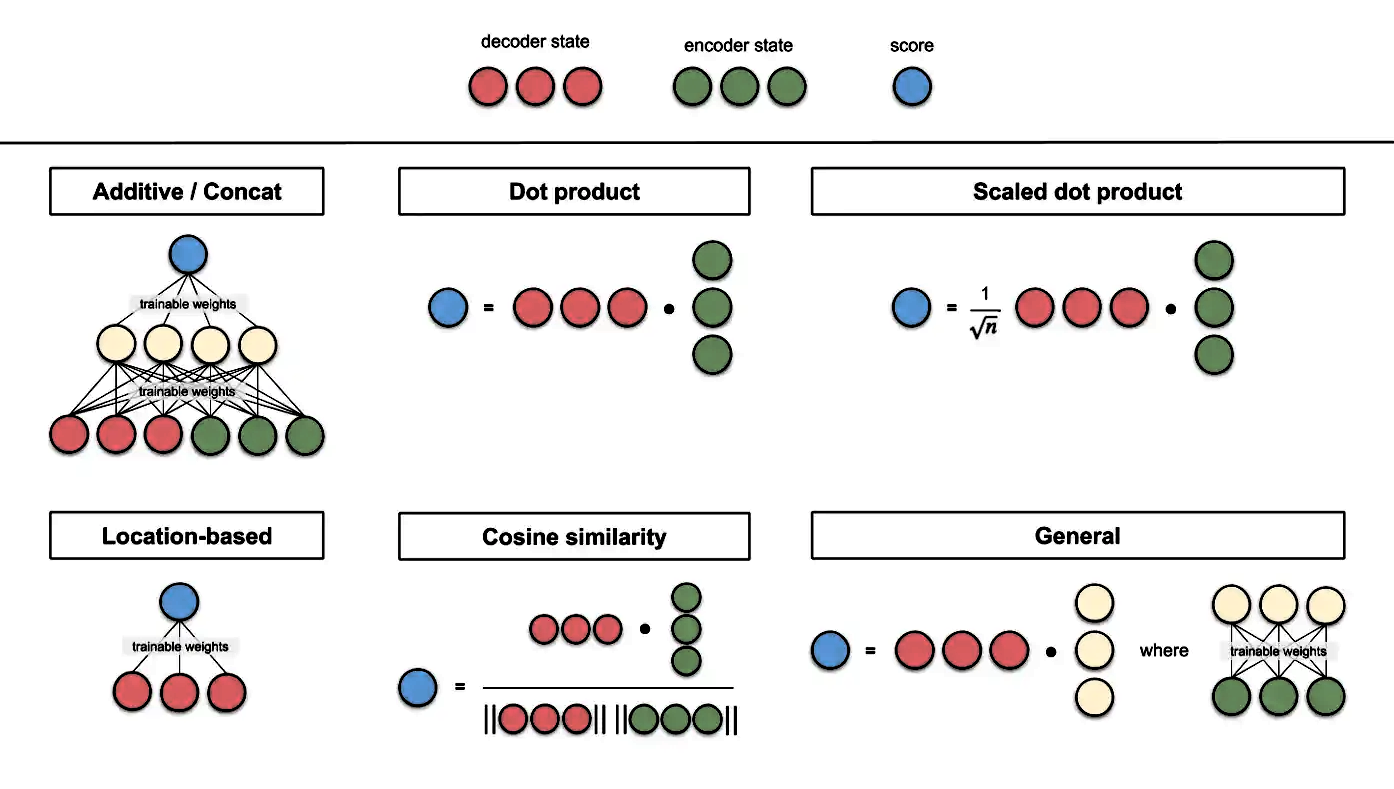
\includegraphics[width=\textwidth]{images/attention_types}}
 	\caption{\textRL{أنواع توابع الانتباه}
 	\textLR{\cite{IllustratedAttention}}}
 	\label{fig:att_types}
 \end{figure}

\begin{itemize}
	\item الانتباه الجمعي 
	$score(A,B) = v_\alpha^T tanh(W_a[A;B])$
	\item
	انتباه الجداء السلمي 
	$score(A,B) = A^TB$
	\item
	انتباه الجداء السلمي المقيس
	$score(A,B) = \frac{A^TB}{\sqrt{ns}}$
	وهو النوع المستخدم في نموذج المحول 
	\textLR{\cite{Vaswani17}}،
	حيث
	$n$
	هي بعد الشعاع
	$B$.
	\item الانتباه المعتمد على المحتوى
	$score(A,B) = cosine[A,B] = \frac{A.B^T}{||A||.||B||}$ 
	
	\item
	الانتباه العام
	$score(A,B) = A^TW_aB$


	
\end{itemize}
\section{المحول في الرؤية الحاسوبية}
في هذه الفقرة سنذكر استخدامات نموذج المحول في مجال الرؤية الصنعية، إذ بسبب النجاح الذي حققه المحول في تطبيقات معالجة اللغات الطبيعية، فقد استخدم في مجالات الرؤية الحاسوبية في السنوات الأخيرة، وقدأعطى نتائج تفوقت على أحدث وأفضل الخوارزميات في هذا المجال بالنسبة للعديد من معايير التقييم في هذا المجال مثل 
\textLR{Imagenet, coco}
وغيرها
\textLR{\cite{ViTsurvey}}.
فقد تم استخدام المحول في مجال توليد
\textLR{\cite{Transgan}}،
تصنيف
\textLR{\cite{ViT}}،
كشف
\textLR{\cite{DETR}}،
وتحسين الصور
\textLR{\cite{Pre-trainedimageTransformer}}،
تصنيف الفيديو
\textLR{\cite{Non-local neural networks}}،
والملاحقة
\textLR{\cite{transformertracker}}،
والذي هو موضوع بحثنا.
\newline
سنتكلم بإيجاز في هذه الفقرة عن النماذج الأولى والأساسية التي استخدمت المحول في مجال الرؤية الصنعية وهي نموذج
\textLR{ViT\cite{ViT}}
ونموذج
\textLR{DETR\cite{DETR}}.
وقد ظهرت بعدها الكثير من النماذج التي اعتمدت على المحول في تطبيقات الرؤية الحاسوبية.
\subsection{المحول والشبكات التلافيفية}
ذكرنا في فقرة سابقة 
\ref{section:transformer}
أن المحول استغنى عن شبكات 
\textLR{RNN}
والتي كانت الأكثر استخداما في مجال معالجة اللغات الطبيعية
\textLR{\cite{Vaswani17}}،
وتحدثنا عن المشكلات التي تعاني منها هذا النوع من الشبكات ذات المعالجة التسلسلية. أما فيما يخص الرؤية الحاسوبية فإن شبكات
\textLR{CNN}
هي الأكثر استخداماً، وهي على العكس من شبكات 
\textLR{RNN}
يمكن بفعالية أن تعالَج بشكل تفرعي باستخدام  
\textLR{GPU}.
ولكن حتى الآن فإن الكثير من الأبحاث لم تستبدل شبكات
\textLR{CNN}
بنموذج المحول بشكل كلي بالرغم من تفوق المحول في الأداء عند تدريبه على معطيات كافية. والسبب في ذلك يعود إلى محاسن شبكات 
\textLR{CNN}
من حيث المحلية
\textLR{locality}،
أي أخد البكسلات المجاورة بعين الاعتبار عند المعالجة كما سنذكر لاحقاً.
\subsubsection{ميزات الشبكات التلافيفية}
\begin{itemize}
\item
غير متغيرة مع الانسحاب
\item
تأخذ العمليات الحسابية في هذه الشبكات المناطق المحلية بعين الاعتبار، فبالتالي السمات المستخرجة منها حساسة محلياً وتحمل معلومات مكانية بشكل أكبر من المحول.
\item
وبسبب هذه الميزة وهي المحلية،
فإن
\textLR{CNN}
جيدة لاستخراج السمات من الصورة، ولكن ليست قادرة على نمذجة العلاقات أو الارتباطات بين هذه السمات، وبالتالي تفتقر إلى الفهم العام للصورة. أما بالنسبة للمحول فإن نقطة قوته هي القدرة على فهم السياق العام
\textLR{\cite{TransformerCV}}،
والنمذجة بشكل
\textLR{global}
أي نمذجة العلاقات الطويلة الأمد بين السمات
\textLR{long-range dependencies}
\textLR{\cite{Swin Transformer V1 and V2}}.
\end{itemize}
بعض الأعمال استخدمت المحول في مجال الرؤية الحاسوبية وقد أعطت نتائج تفوقت على الخوارزميات الرائدة في هذا المجال عند وجود عدد كافي من معطيات التدريب، وذلك بالاعتماد فقط على توابع الانتباه ودون أي استخدام للشبكات التلافيفية 
\textLR{\cite{ViT}}،
بالرغم من أن هذه النماذج لها بنية أبسط، وتستهلك زمن تدريب أقل مقارنة بنماذج الشبكات التلافيفية
\textLR{\cite{TransformerCV}}.
\subsection{المحول في مجال التصنيف}
ظهرت العديد من خوارزميات التصنيف التي تستخدم المحول في السنوات الأخيرة، بعضها قد حسن الخوارزميات المعتمدة على الشبكات التلافيفية بإضافة أجزاء من المحول إليها، وذلك كونه ينمذج الترابطات الطويلة الأمد، مثل
\textLR{VT\cite{VT}}،
\textLR{BotNet\cite{BotNet}}.
وكون البنية الأصلية للمحول 
\textLR{\cite{Vaswani17}}
تهمل المعلومات المحلية، لذلك كان هنالك العديد من التحسينات على بنية
\textLR{ViT\cite{ViT}}،
من هذه التحسينات إضافة أجزاء من الشبكات التلافيفية لتحسين المحول، مثل خوارزمية
\textLR{BEiT\cite{BEiT}}،
وخوارزمية 
\textLR{ConViT\cite{ConViT}}.
\newline
وهناك تحسينات أخرى مثل المحول الذي يعتمد على الانتباه المحلي،
هذه الخوارزميات قد أعادت تصميم تجزئة الصورة 
\textLR{patch partition}،
وأعادت تصميم كتل توابع الانتباه بهدف إضافة المعلومات المحلية(المكانية) إلى المحول، دون الاعتماد على الشبكات التلافيفية وذلك مثل خوارزمية 
\textLR{TNT\cite{TNT}}،
\textLR{Volo\cite{Volo}},
و 
\textLR{SwinTransformer\cite{swintransformer}}
والتي سنتحدث عنها في الفقرة
\ref{section:swinTransformer}
كونها الـ
\textLR{backbone}
المستخدم في نموذجنا.
\newline
عدلت العديد من الأبحاث بنية المحول  إلى بنية هرمية وعميقة مثل
\textLR{T2T-ViT\cite{T2T-ViT}}،
\textLR{PVT\cite{PVT}}،
وذلك محاكاة لبنية الشبكات التلافيفية الهرمية والعميقة 
\textLR{\cite{Why Deep Learning Works}}.
\newline
بحسب المقالة
\textLR{\cite{ViTsurvey}}،
والتي تقارن وتصنف أكثر من مئة محول في مجال الرؤية الحاسوبية فإن الأبحاث الحديثة لا تميل إلى استخدام البنية الأصلية للمحول، ولم تستغني عن استخدام الشبكات التلافيفية بشكل كامل، بل العكس من ذلك استخدام البنية الهجينة هو ما يعطي أفضل النتائج، بالرغم من أن المحول يمكن أن يوازي بأداءه الشبكات التلافيفية أو حتى يفوقها في الأداء، ويعود ذلك إلى أن المعلومات المحلية مهمة جداً لتحسين أداء المحول كما في 
\textLR{Volo\cite{Volo}}،
و
\textLR{SwinTransformer\cite{swintransformer}}،
وهما نسخة المحول الأكثر استخداما في الرؤية الحاسوبية.
في هاتين الخوارزميتين تم استخدام خليط من المعلومات العامة 
\textLR{global}
والمعلومات المحلية 
\textLR{local}.
\newline
أما على صعيد تحسين الاجزاء الأخرى من المحول مثل تحسين الترميز المكاني
\textLR{Positional Encoding PE}
فهناك العديد من الأبحاث مثل
\textLR{\cite{Conditional positional encodings for ViT}}،\textLR{\cite{RethinkingPE}}،\textLR{\cite{deeper look at position information in cnns}}. 
أو تحسين بنية
\textLR{MHA}
الانتباه متعدد الرؤوس
\textLR{\cite{Cordonnier}}،
أو تحسين 
\textLR{MLP}
كما في 
\textLR{\cite{Attention is not all you need}}.
\subsection{المحول في مجال الكشف}
أول خوارزمية استخدمت المحول في مجال الكشف هي 
\textLR{DETR\cite{DETR}}،
استخدمت هذه الخوارزمية تمثيل جديد وهو
\textLR{object query}،
وهو أحد مداخل مفكك الترميز،
وهو مجموعة من الأوزان القابلة لتعلم السمات العامة في الصورة. كان هناك العديد من التحسينات على هذه الخوارزمية مثل
\textLR{DeformableDETR\cite{DeformableDETR}}،
و
\textLR{ACT\cite{ACT}}،
كون الخوارزمية الأصلية
\textLR{\cite{DETR}}
تعاني من دقة كشف منخفضة من أجل الأغراض الصغيرة وتأخذ زمن طويل في التدريب.
\newline
هناك العديد من الدراسات التي أعادت تصميم بنية المحول مثل
\textLR{TSP\cite{TSP}},
\textLR{YOLOS\cite{YOLOS}}.
أو باستخدام المحول كـ
\textLR{backbone}
لاستخلاص السمات من الصورة كما في
\textLR{FPT\cite{FPT}}.
\subsection{خوارزمية التصنيف
\textLR{ViT\cite{ViT}}}
هذه الخوارزمية لا تستخدم الشبكات التلافيفية في بنيتها. إذ يتم تقسيم الصورة إلى أقسام عدة
\textLR{patches}،
كل قسم
\textLR{patch}
يعامل معاملة ال 
\textLR{token}
(الكلمة) في المحول الأصلي، أي يتم إدخاله إلى طبقة
\textLR{embedding}
خطية لتحويله إلى شعاع بأبعاد مختلفة.
\newline
عند تدريب هذا النموذج على معطيات تدريب ذات حجم متوسط مثل
\textLR{ImageNet}
كان أداؤه متواضع وأقل من أداء نموذج
\textLR{ResNet\cite{ResNet}}
و بعدد أوزان متقارب. لكن النتائج تغيرت عند تدريبه على معطيات تدريب بحجوم كبيرة ( 
$14$
مليون -
$300$ 
مليون عينة) مثل 
\textLR{ImageNet-21K},
\textLR{JFT-300M}،
عندها أعطى النموذج نتائج تفوقت على الخوارزميات السابقة.
\newline
دخل النموذج الأصلي للمحول هو سلسلة ببعد واحد . للتعامل مع الصورة وللمحافظة على البنية الأساسية للمحول فقد  تم تعديل الصورة
$x\in \mathds{R}^{H\mathsf{x}W\mathsf{x}C}$
وتحويلها إلى سلسلة من الأجزاء المسطحة
$x_p \in  \mathds{R}^{N\mathsf{x}(P^2.C)}$
ذات بعد واحد، وذلك لمحاكاة دخل المحول الأصلي. حيث
$H\mathsf{x}W$
أبعاد الصورة،
$C$
عدد القنوات والتي هي في الغالب
$RGB = 3$،
$P\mathsf{x}P$
أبعاد كل قسم من الصورة
\textLR{patch}،
$N$
 عدد الأقسام أو الأجزاء
$N = \frac{HW}{P^2}$.
\newline
يتم إدخال الشعاع 
$x_p$
إلى طبقة إسقاط خطي أي شبكة عصبونية بطبقة واحدة مع تابع تفعيل خطي، وذلك لتحويل أبعاده إلى 
$(N,D)$
كما في المعادلة
\ref{eq:vit1}.
\begin{equation}
z_0 = [x_{class};X_p^1E;x_p^2E;...;x_p^NE]+E_{pos},	E\in \mathds{R}^{(P^2.C)\mathsf{x}D},E_{pos}\in \mathds{R}^{(N+1)\mathsf{x}D}
\label{eq:vit1}
\end{equation}
\begin{equation}
Z_l^\prime = MSA(LN(z_{l-1})) + z_{l-1},	l = 1 ... L
\label{eq:vit2}
\end{equation}
\begin{equation}
Z_l = MLP(LN(z_l^\prime)) + z_l^\prime,	l = 1 ... L
\label{eq:vit3}
\end{equation}
\begin{equation}
y = LN(z_L^0)
\label{eq:vit4}
\end{equation}
حيث
$D$
هو
\textLR{hyperparameter}
ويمكن تسميته ببعد الـ
\textLR{embedding}.
$E$
هي طبقة الإسقاط الخطي، بعدد بارامترات
$E \in \mathds{R}^{(P^2.C)\mathsf{x}D}$
قابلة للتدريب.
وكما في خوارزمية
\textLR{BERT\cite{BERT}}
فيتم إضافة شعاع من البارامترات ندعوه بالـ
\textLR{class token}
قابل للتدريب بأبعاد
$(1\mathsf{x}D)$،
وهو 
$x_{class}$
في المعادلة 
\ref{eq:vit1}.
 حيث يتم اعتبار أن حالة هذا الشعاع في الخرج النهائي للمحول
$z_L^0$
يمكن تدريبها لتعبر عن صنف الصورة، وذلك بعد تعديل هذا الشعاع بإدخاله إلى شبكة التصنيف
\textLR{classification head}.
$L$
هي عدد طبقات المرمز.
\newline
نضيف إلى هذا الشعاع شعاع ترميز الموقع 
$E_{pos}$
وذلك لإدخال المعلومات المكانية النسبية بين أجزاء الصورة، استخدمت
\textLR{ViT}
ترميز موقع ببعد واحد قياسي.
$Z_0$
هو دخل المحول كما في المعادلة
\ref{eq:vit1}.
\newline
يستخدم
\textLR{ViT}
بنية مرمز مطابقة لبنية المرمز في المحول الأصلي من حيث توابع انتباه متعددة الرؤوس كما في المعادلة 
\ref{eq:vit2}
وشبكة
\textLR{MLP}
كما في المعادلة 
\ref{eq:vit3},
ويتم تطبيق طبقة تقييس قبل كل كتلة، بالإضافة إلى 
\textLR{residual connections\cite{residual}}
بعد كل كتلة. وكما يوضح الشكل
\ref{fig:ViT}

\begin{figure}[h!]
	\centerline{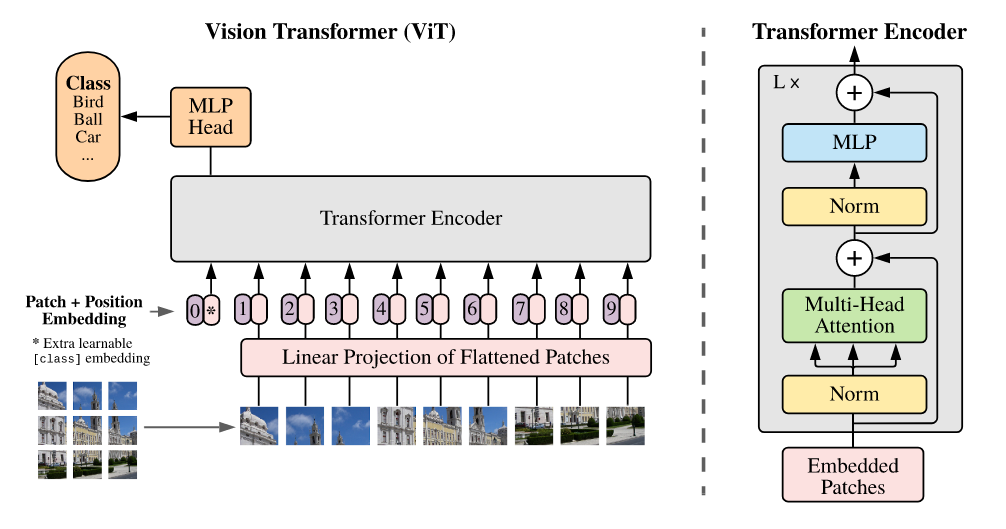
\includegraphics[width=\textwidth]{images/ViT}}
	\caption{
	\textRL{بنية خوارزمية}
	\textLR{ViT}
	\textLR{\cite{ViT}}}
	\label{fig:ViT}
\end{figure}

\subsection{خوارزمية الكشف
	\textLR{DETR\cite{DETR}}
\label{section:detr}}

\begin{figure}[h!]
	\centerline{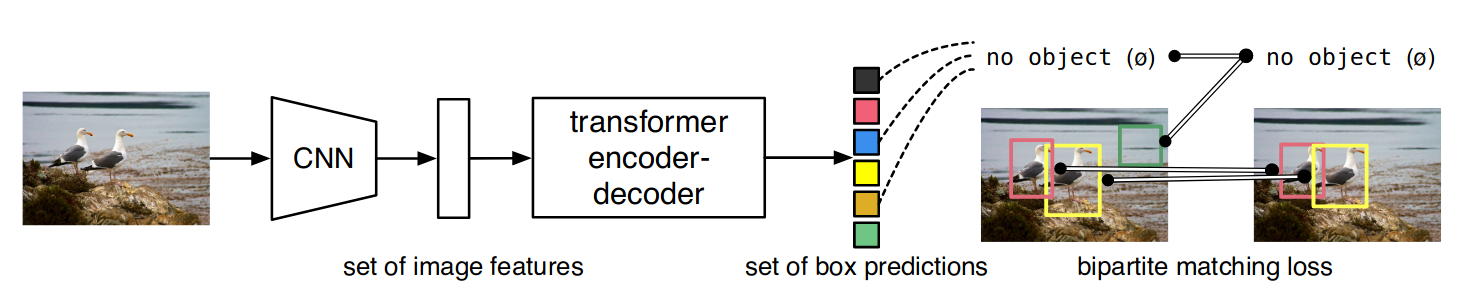
\includegraphics[width=\textwidth]{images/DETR}}
	\caption{\textRL{بنية الكاشف}
	\textLR{DETR}
	\textLR{\cite{DETR}}}
	\label{fig:DETR}
\end{figure}
\selectlanguage{arabic}
كما يوضح الشكل
\ref{fig:DETR}
فإن النموذج يستخدم شبكة تلافيفية كـ
\textLR{backbone}
 لاستخلاص السمات من الصورة التي أبعادها
$x_{img} = \in \mathds{R}^{3\mathsf{x}H_0\mathsf{x}W_0}$،
وأبعاد خريطة السمات بعد الشبكة التلافيفية
$f \in \mathds{R}^{C\mathsf{x}H\mathsf{x}W}$،
حيث
$H,W = \frac{H_0}{32},\frac{W_0}{32}$
و
$C = 2048$.
يتم تخفيض الأبعاد من $C$ إلى  $d$، وتحويل خريطة السمات من بعدين إلى بعد واحد عبر التسطيح
\textLR{flattening}
 فيصبح لدينا أبعاد دخل المرمز
$N\mathsf{x}d$
حيث
$N=H\mathsf{x}W$.
\newline
ونلاحظ أيضا أن الخوارزمية قد اتبعت بنية المحول الأصلي أي بنية مرمز-مفكك ترميز مع فوارق بسيطة مثل دخل مفكك الترميز. في  المحول الأصلي دخل مفكك الترميز هو الخرج في اللحظة الزمنية السابقة، أما في 
\textLR{DETR} 
فهو عبارة بارامترات قابلة للتدريب تدعى
\textLR{object queries}،
تعبر عن ترميز مكاني لكل غرض ويتم فك هذا الترميز عبر مفكك الترميز.
نلاحظ أن كل من الخوارزميتين السابقتين 
\textLR{ViT}
و
\textLR{DETR}
استخدمتا بنية المحول الأصلي مع تعديلات بسيطة. أما بالنسبة  للخوارزمية التي استخدمناها لاستخلاص السمات في نموذجنا وهي محول
\textLR{Swin\cite{swintransformer}}،
والتي سنتحدث عنها في الفقرة التالية فقد عدلت بشكل كبير في بنية المحول.

\subsection{المحول في الملاحقة}
في عام 
$2021$
بدأت تظهر أنظمة ملاحقة تستخدم المحول في بنيتها، سنذكر في هذه الفقرة بعض من تطبيقات المحول في مجال الملاحقة.
\newline
فمثلا استخدمت خوارزمية 
\textLR{TransT\cite{transformertracker}}
الطريقة الموضحة في الشكل 
\ref{fig:TransT}،
بداية تُستخدم شبكة 
\textLR{ResNet-50\cite{ResNet}}
لاستخلاص السمات من صورتي الغرض ومنطقة البحث، ومن ثم تستخدم كتلة انتباه ذاتي لكل من سمات الصورتين، مسماة في الورقة البحثية بـ
\textLR{ECA Ego-Context Augment Modules}
موضحة في المخطط اليسار من الشكل 
\ref{fig:TransT_Modules}.
ويتم دمج هذه السمات عبر كتلة انتباه تقاطعي تدعى بـ
\textLR{CFA Cross-Feature Augment Module}.
يتم الدمج عبر ثلاث مراحل موضحة في الشكل 
\ref{fig:TransT}
\begin{itemize}
	\item
	دمج خرج كتلة 
	\textLR{ECA}
	للغرض باعتبارها 
	\textLR{query}
	 ولمنطقة البحث باعتبارها
 	\textLR{key,value}.
 	\item
 	دمج بتبديل المداخل أي باعتبار سمات الغرض هي 
 	\textLR{key,value}
 	وسمات نافذة البحث هي 
	\textLR{query}.
 	\item
 	دمج الخرجين السابقين ضمن كتلة 
	\textLR{ECA}
	ثالثة.
\end{itemize}
مع إضافة ترميز مكاني إلى كل من 
\textLR{key,query}
في كل كتلة.
\newline

\begin{figure}[!h]
	\centerline{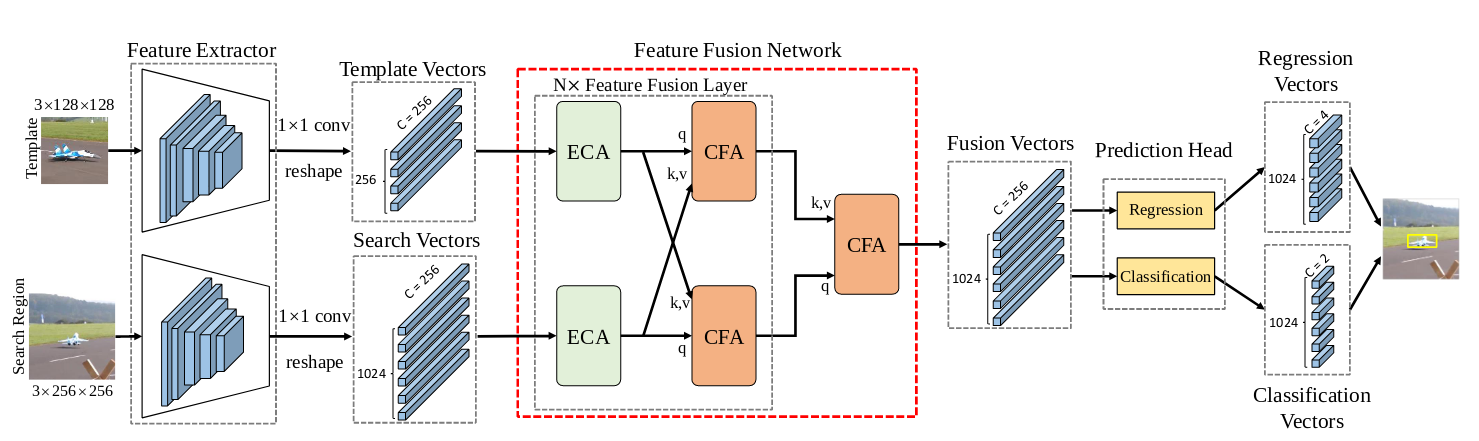
\includegraphics[width=\textwidth]{images/TransT}}
	\caption{
		\textRL{بنية خوارزمية الملاحقة}
		\textLR{TransT}
		\textLR{\cite{transformertracker}}}
	\label{fig:TransT}
\end{figure}

\begin{figure}[!h]
	\centerline{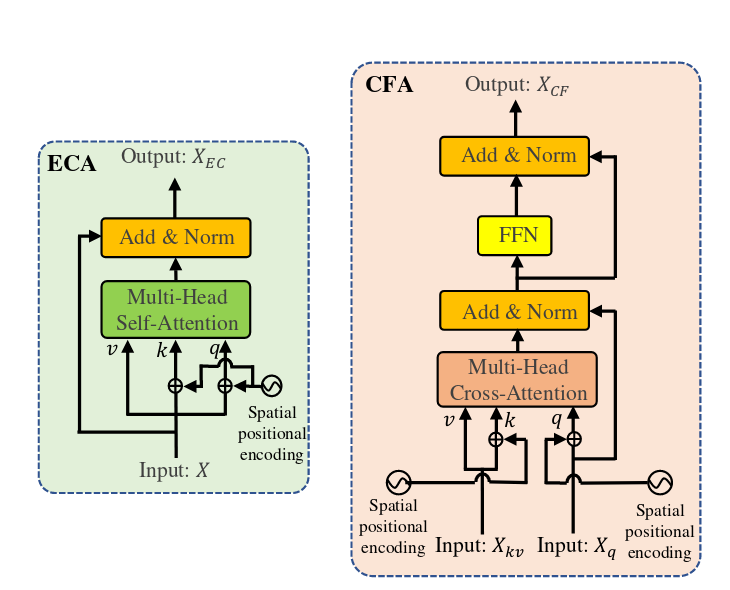
\includegraphics[scale=0.4]{images/TransT_ECA_CFA.png}}
	\caption{
		\textRL{بنية خوارزمية الملاحقة}
		\textLR{TransT}
		\textLR{\cite{transformertracker}}}
	\label{fig:TransT_Modules}
\end{figure}
كما أن خوارزمية الملاحقة
\textLR{TrTr\cite{TrTr}}
تستخدم بنية شبيهة ببنية المحول الأصلي كما يوضح الشكل 
\ref{fig:TrTr}،
بحيث يكون دخل المرمز هو سمات صورة الغرض الإبتدائية، ويطبق الانتباه الذاتي للتركيز على السمات المهمة. بينما يكون دخل مفكك الترميز هو سمات نافذة البحث ويطبق عليها تابع انتباه ذاتي، والدخل الثاني هو خرج المرمز (سمات الغرض المعدلة)، ويتم تطبيق تابع الانتباه التقاطعي بين الدخلين.
\begin{figure}[!h]
	\centerline{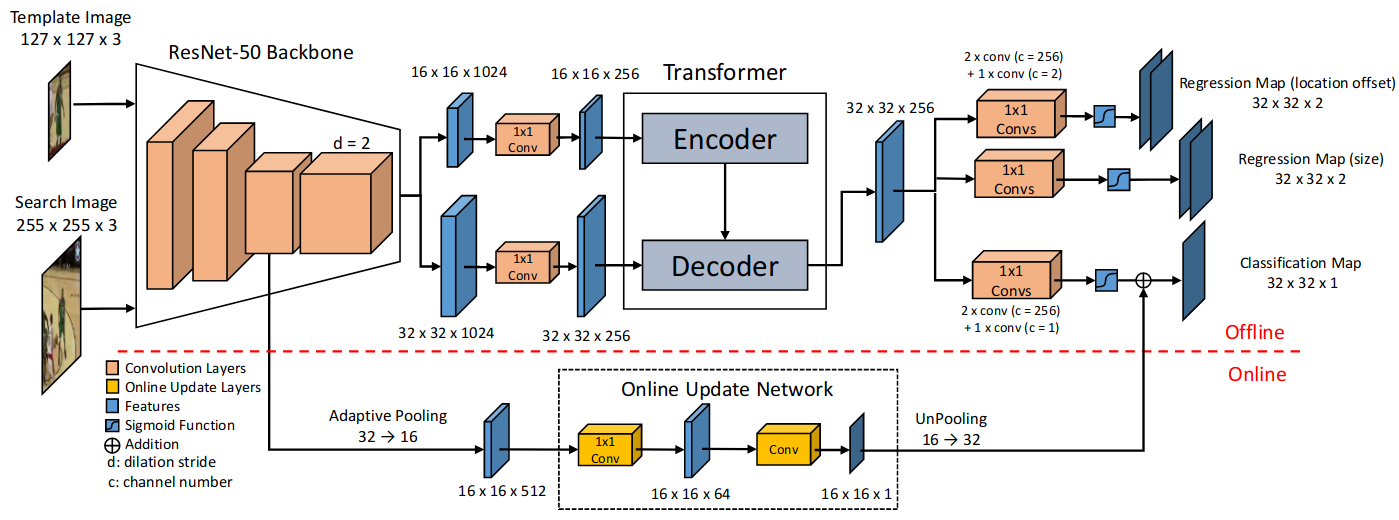
\includegraphics[width=\textwidth]{images/TrTr.png}}
	\caption{\textRL{بنية خوارزمية الملاحقة}
	\textLR{\cite{TrTr}}
	\textLR{TrTr}}
	\label{fig:TrTr}
\end{figure}
\newline
بالإضافة إلى خوارزميتي الملاحقة السابقتين فهناك خوارزمية الملاحقة 
\textLR{STARK\cite{Stark}},
وخوارزمية الملاحقة 
\textLR{SwinTrack\cite{swinTrack}}،
واللتان سيتم شرحهما بالتفصيل في الفصل القادم.
%وقد تم الاعتماد عليهما في البحث، وسيتم شرحهما بالتفصيل في الفصل القادم.
ويجب أن نلاحظ بمقارنة الخوارزميات الأربعة السابقة ببعضها بأن كل من 
\textLR{TransT\cite{transformertracker}}
و
\textLR{TrTr\cite{TrTr}}
تقوم بمعالجة سمات الغرض وسمات نافذة البحث على حدة ضمن توابع الانتباه، بينما في خوارزميات الملاحقة 
\textLR{SwinTrack\cite{swinTrack}}
و
\textLR{STARK\cite{Stark}}
كما سنرى لاحقاً،
فإنها تقوم بضم أشعة السمات للصورتين ضمن شعاع واحد، وتعتبره كدخل للمرمز.
\newline
هذا فيما يتعلق بخوارزميات الملاحقة لغرض واحد والتي تستخدم نموذج المحول ضمن بنيتها، وبمقارنة هذه الخوارزميات بسابقتها والتي لا تستخدم المحول، فنلاحظ كما يوضح الشكل
\ref{fig:comapre}،
والذي يقارن عدة خوارزميات ملاحقة حديثة من ناحية الأداء والسرعة على مجموعة المعطيات الخاصة بالملاحقة 
\textLR{LaSOT\cite{Lasot}}،
بأن خوارزميات الملاحقة التي تستخدم المحول حققت أفضل أداء وسرعة مقارنةً بغيرها من الخوارزميات، وهذا ماشجعنا على اعتمادها في البحث.
وبمقارنة الخوارزميات الأربعة السابقة بالنسبة لبعضها فنلاحظ من الجدول 
\ref{table:compare__trans_trackers}،
والذي يقارن هذه الخوارزميات من أجل مجموعة المعطيات 
\textLR{LaSOT\cite{Lasot}}،
بأن أفضل أداء حققته خوارزمية 
\textLR{SwinTrack\cite{swinTrack}}، 
يليها خوارزمية 
\textLR{STARK\cite{Stark}}،
وبسبب تفوق خوارزمية 
\textLR{SwinTrack\cite{swinTrack}}
في الأداء والسرعة، قررنا أن نعتمدها في بحثنا.
\vspace{-5.0mm}
\begin{figure}[H]
\centerline{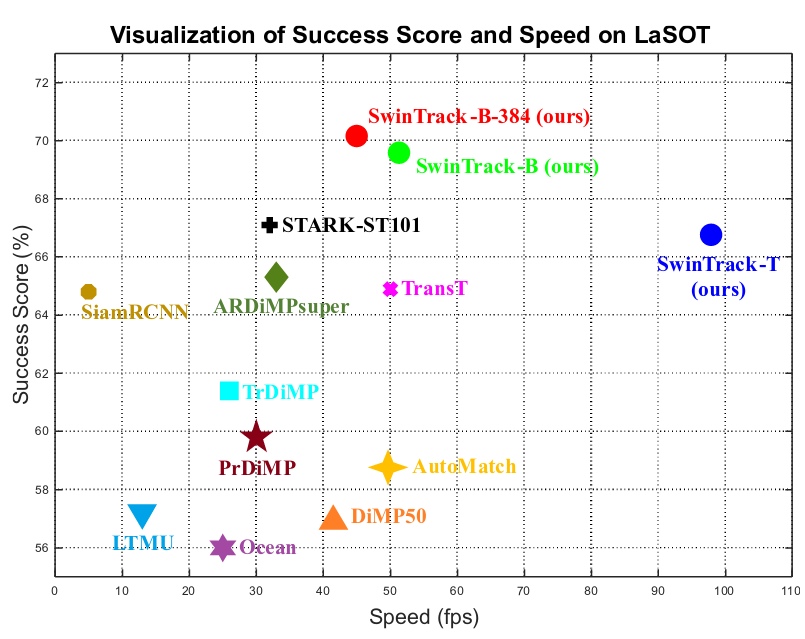
\includegraphics[width=0.6\textwidth]{images/transformerInTrackingComapre.png}}
	\caption{\textRL{
			مقارنة بين بعض الخوارزميات التي تستخدم المحول مع خوارزميات
	}}
	\label{fig:comapre}
\end{figure}
\vspace{-7.0mm}
\centerline{\textRL{
		الملاحقة الأخرى  من ناحية السرعة و الأداء على مجموعة المعطيات
			 \textLR{LaSOT\cite{Lasot}}
		\textLR{\cite{swinTrack}}
}}	

%\begin{figure}[!h]
%	\centerline{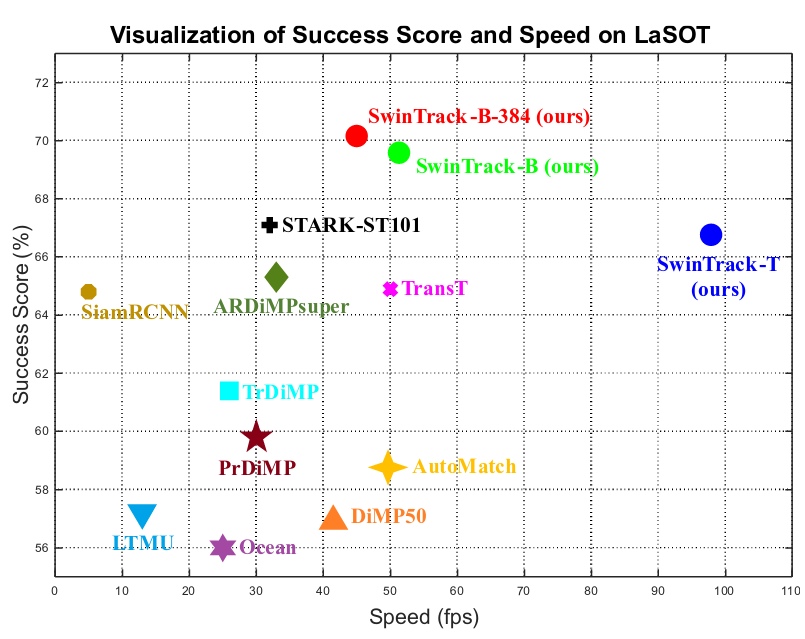
\includegraphics[width=0.6\textwidth]{images/transformerInTrackingComapre.png}}
%	\caption{
%		\textRL{مقارنة بين بعض الخوارزميات التي تستخدم المحول مع خوارزميات الملاحقة الأخرى
%			 من ناحية السرعة و الأداء على مجموعة المعطيات}
%		 \textLR{LaSOT\cite{Lasot}}
%		\textLR{\cite{swinTrack}}
%		}
%	\label{fig:comapre}
%\end{figure}

\begin{table}[H]
	\centering
	\begin{tabular}{c c c c c c c} 
		\hline
		\textLR{Tracker} & \textLR{AUC}\% & \textLR{Normalized Precision} & \textLR{Precision}&\textLR{Year}\\ [0.5ex] 
		\hline\hline
		\textLR{SwinTrack-B-384} &$70.2$&$78.4$&$75.3$&$2021$\\
		\textLR{STARK} & $67.1$ & $77.0$ &&$2021$\\ 
		\textLR{TransT} &$64.9$ & $73.8$ & $69.0$&$2021$\\
		\textLR{TrTr} & $55.1$ &&&$2021$&\\[1ex] 
		\hline
	\end{tabular}
	\caption{
		\textRL{مقارنة بين خوارزميات الملاحقة السابقة}}
	\label{table:compare__trans_trackers}
\end{table}
\vspace{-8.0mm}
\centerline{\textRL{
		\textRL{من أجل معطيات التدريب}
\textLR{LaSOT\cite{Lasot}}	
}}	
أما فيما يتعلق بالملاحقة لعدة أغراض فهناك خوارزمية 
\textLR{TrackFormer\cite{TrackFormer}}
والتي استخدمت بنية محول مشابهة لخوارزمية
\textLR{TrTr\cite{TrTr}},
بينما استخدمت خوارزمية
\textLR{TransTrack\cite{TransTrack}}
سمات الإطار الحالي والإطار السابق كدخل للمرمز مع استخدام كتلتي مفكك ترميز،
دخل مفكك الترميز هو
\textLR{object query} 
قابلة للتدريب، وذلك كما في خوارزمية 
\textLR{DETR\cite{DETR}}
المشروحة في الفقرة 
\ref{section:detr}.
\subsection{المحول 
\textLR{Swin}\label{section:swinTransformer}}
صمم المحول الأصلي ليناسب تطبيقات معالجة اللغات الطبيعية، وبسبب اختلاف هذا المجال عن مجال الرؤية الحاسوبية، ظهرت العديد من الدراسات لتعديل بنية المحول لتتناسب مع مجال الرؤية.
\newline
نذكر بعض الاختلافات بين المجالين
\begin{itemize}
	\item
	في تطبيقات معالجة اللغات الطبيعية فإن الكلمة التي نحولها إلى 
\textLR{token}
	 هي العنصر الأساسي. وكل الـ
\textLR{tokens}
لها نفس الحجم، أما بالنسبة للتطبيقات الرؤية الحاسوبية فإن الأغراض في الصورة أو العناصر المرئية
\textLR{visual elements}
لها حجوم ومقاييس
\textLR{scales}
مختلفة. بعض خوارزميات الكشف قد عالجت مشكلة اختلاف مقاييس الأغراض مثل
\textLR{\cite{Feature pyramid networks for object detection}},
\textLR{\cite{An analysis of scale invariance in object detection}}.
\item
العدد الكبير للبكسلات في الصورة مقارنة بعدد الكلمات في الجملة، وهذا ما يجعل المحول الأصلي ذا تعقيد حسابي كبير من أجل المهمات التي تتطلب معالجة على مستوى البكسل مثل 
\textLR{semantic segmentation}،
أو من أجل الصور ذات الحجوم الكبيرة، حيث يكون التعقيد الحسابي للانتباه الذاتي متناسب بشكل تربيعي مع حجم الصورة.
\end{itemize}
\subsubsection{إشكالية نموذج
\textLR{ViT\cite{ViT}}
ونموذج المحول الأصلي 
\textLR{\cite{Vaswani17}}}
بالرغم أن خوارزمية
\textLR{ViT\cite{ViT}}
لم تعدل على بنية المرمز الأصلي للمحول، إذ أنها فقط جزأت الصورة إلى
$16 \mathsf{x} 16$
جزء 
\textLR{patch}،
إلا أنها تفوقت على أفضل المصنفات حين تم تدريبها على معطيات تدريب كافية 
\textLR{JFT-300M}،
لكن الـ 
\textLR{tokens}
في
\textLR{ViT}
كان لها حجم ومقياس ثابت، وهذا كما ذكرنا في الفقرة السابقة، غير مناسب لأغراض الرؤية الحاسوبية.
المشكلة الأخرى عندما تكون صورة الدخل ذات دقة عالية يزداد التعقيد الحسابي بشكل تربيعي مع زيادة حجم الصورة. وأيضا كل من
\textLR{ViT} 
والنموذج الأصلي
\textLR{\cite{Vaswani17}} 
غير مناسب للتطبيقات التي تحتاج معالجة على مستوى البكسل بسبب التعقيد الحسابي العالي، إذ يتم حساب تابع الانتباه بين الـ
\textLR{tokens}
كلها.
\subsubsection{نموذج
\textLR{Swin}}
كما ذكرنا فإن محول
\textLR{Swin}
هو النموذج المستخدم لاستخراج السمات، وسنبين في هذه الفقرة اختلافه عن المحول الأصلي، وسبب تفوقه من ناحية الأداء والسرعة، وهذا ماجعله مناسب لبحثنا كوننا نهتم بتطبيقات الزمن الحقيقي.
\newline
نموذج محول 
\textLR{Swin}
اختصار لـ
\textLR{Shifted Windows Transformer}،
أي نموذج محول مع نوافذ مزاحة،
وهو نموذج هرمي
\textLR{hierarchical}،
إذ يسمح بالنمذجة من أجل مقاييس متنوعة. بالإضافة إلى أنه يقسم الصورة إلى نوافذ 
\textLR{windows}،
ويحسب الانتباه بين الأجزاء ضمن النافذة الواحدة، وهذا ما يجعل التعقيد الحسابي خطي بالنسبة لحجم الصورة، كونها تحد حساب الانتباه الذاتي ضمن نوافذ غير متقاطعة.
أما بالنسبة للنوافذ غير المتقاطعة فإن طريقة النوافذ المزاحة 
\textLR{shifted-windows}
تسمح باتصال النوافذ ببعضها.
\begin{figure}[!h]
	\centerline{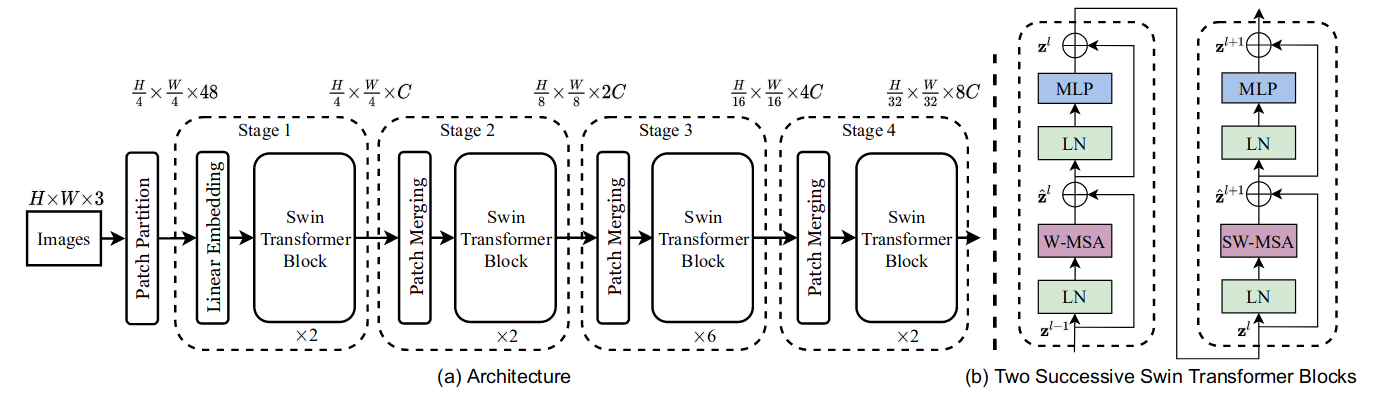
\includegraphics[width=\textwidth]{images/swin_architecture}}
	\caption{
	\textRL{بنية محول}
	\textLR{Swin-Tiny}
	\textLR{\cite{swintransformer}}}
	\label{fig:swin}
\end{figure}
\newline
يبين الشكل 
\ref{fig:swin}
 بنية المحول
\textLR{Swin-Tiny}،
وكما نلاحظ فإن الجزء الأول من المخطط هو
\textLR{patch partition}،
إذ يتم تقسيم الصورة إلى أجزاء 
\textLR{patches}
كما في خوارزمية
\textLR{ViT\cite{ViT}}،
%وهو كما يوضح الشكل
%\ref{fig:swin_patch_partition}،
%يتم بداية تقسيم الصورة إلى نوافذ وهي الخطوط الحمراء في الشكل، وكل نافذة تقسم إلى أجزاء
%\textLR{patches}
%وهي الخطوط الرمادية  كما في خوارزمية
%\textLR{\cite{ViT}}،
%\begin{figure}[!h]
%	\centerline{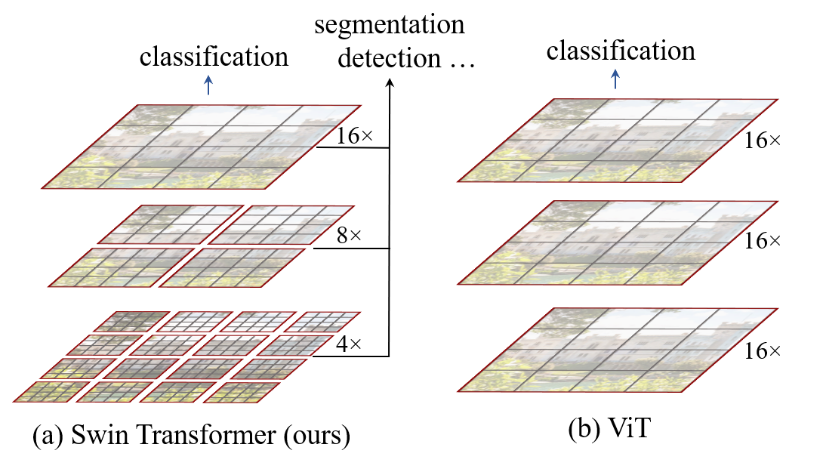
\includegraphics[width=\textwidth]{images/swin_patch_patition.png}}
%	\caption{
%	\textRL{الفرق بين تقسيم النوافذ بين محولي}
%	\textLR{ViT\cite{ViT},Swin\cite{swintransformer}}}
%	\label{fig:swin_patch_partition}
%\end{figure}
حيث يعامل كل جزء معاملة
\textLR{token}،
حجم كل جزء
$4\mathsf{x}4\mathsf{x}3 = 48$،
وبالتالي عدد عناصر سلسلة الدخل أو عدد الـ
\textLR{tokens}
هو
$(\frac{H}{4} \mathsf{x} \frac{W}{4})$.
فيكون دخل المرحلة الأولى
\textLR{stage1}
هو سلسلة بأبعاد
$\frac{HW}{16} \mathsf{x}48$.
\newline
الكتلة الأولى في المرحلة الأولى هي 
\textLR{linear embedding}،
وهي عبارة عن طبقة خطية هدفها إسقاط شعاع السمات السابق إلى بعد 
$C$
أي يصبح
$\frac{HW}{16}\mathsf{x}C$.
ومن ثم يتم تطبيق كتلتي محول 
\textLR{Swin}
متعاقبتين،  بنية الكتلة موضحة في الجزء اليمين من الشكل
\ref{fig:swin}
وسنشرحها في الفقرة القادمة، أبعاد دخل وخرج كتلة محول 
\textLR{Swin}
تبقى ثابتة، أي يكون بعد خرج المرحلة الأولى هو
$\frac{HW}{16}\mathsf{x}C$.
\subsubsection{الهرمية
\textLR{hierarchical}}
نلاحظ بأن الجزء الأول من كل مرحلة تالية هو طبقة
\textLR{patch merging}،
وهو القسم المسؤول عن هرمية النموذج، إذ أن هدف هذه الطبقة الخطية هو تخفيض عدد عناصر سلسلة الدخل أو الـ
\textLR{tokens}،
ويزداد هذا التخفيض  بازدياد عمق النموذج
 كما نلاحظ من أبعاد دخل كل كتلة في الشكل 
\ref{fig:swin}.
\newline
تقوم هذه الطبقة بدمج كل مجموعة
$2\mathsf{x}2$ 
من العناصر المتجاورة وتقوم بسلسلتها فتصبح شعاع واحد بـ$4$ عناصر، وبالتالي يتغير عدد عناصر السلسلة 
فإذا كانت أبعاد السلسلة
$\frac{H}{4}\mathsf{x}\frac{W}{4}\mathsf{x}C$ 
فيصبح
$\frac{H}{8}\mathsf{x}\frac{W}{8}\mathsf{x}4C$،
ومن ثم عبر طبقة خطية تقوم بتغيير أبعاد كل عنصر من السلسلة أو كل 
\textLR{token}
إلى النصف فيصبح
$\frac{H}{8}\mathsf{x}\frac{W}{8}\mathsf{x}2C$،
وهو خرج المرحلة الثانية.
\newline
$\frac{H}{16}\mathsf{x}\frac{W}{16}\mathsf{x}4C$ 
خرج المرحلة الثالثة.
\newline
$\frac{H}{32}\mathsf{x}\frac{W}{32}\mathsf{x}8C$
وهو خرج المرحلة الرابعة والأخيرة في نموذج
\textLR{tiny}.
\newline
إن أبعاد كل مرحلة مشابهة لأبعاد السمات في شبكات
\textLR{CNN}
النموذجية كما في
\textLR{VGG\cite{VGG}, ResNet\cite{ResNet}}
وهذا ما يمكننا من استخدام هذا النموذج كـ
\textLR{backbone}
بديل
لتطبيقات الرؤية الحاسوبية المختلفة.
\subsubsection{كتلة محول
\textLR{Swin}}
نلاحظ من الجزء اليسار من المخطط أن بنية 
\textLR{Swin}
مشابهة لبنية المحول الأصلي، فيما عدا استبدال الانتباه المتعدد الرؤوس 
\textLR{MHA}
بـ انتباه متعدد الرؤوس مع نوافذ
\textLR{W-MHA}
في الكتلة الأولى، وانتباه متعدد الرؤوس مع نوافذ مزاحة 
\textLR{SW-MHA}
في الكتلة التالية.
\subsubsection{التعقيد الحسابي عند استخدام النوافذ}
يوضح الشكل
\ref{fig:swin_shifted_window}
تقسيم النوافذ،
إذ يتم حساب الانتباه الذاتي بين عناصر النافذة الواحدة فقط، وهذا ما يخفض التعقيد الحسابي.
مقارنة بالمحول الأصلي الذي يحسب الانتباه الذاتي بين كل العناصر فإن التعقيد الحسابي من أجل سلسلة دخل بأبعاد 
$hw\mathsf{x}C$ 
يكون: 
\begin{equation}
\Omega(MHA) = 4hwC^2+2(hw)^2C
\end{equation}
نلاحظ أن التعقيد يزداد بشكل تربيعي مع زيادة أبعاد الصورة
بينما في حال استخدام طريقة النوافذ وحساب الانتباه داخل العناصر ضمن النافذة الواحدة فقط فيكون التعقيد الحسابي من أجل كل نافذة تحوي 
$M\mathsf{x}M$ 
جزء أو 
\textLR{patch}
يكون
\begin{equation}
\Omega(W-MHA)=4hwC^2+2M^2hwC
\end{equation}
نلاحظ بأن التعقيد الحسابي متناسب بشكل خطي مع أبعاد الصورة في حال كانت
$M$ 
ثابتة ( في النموذج 
$M=7$
)،
هذا التخفيض في التعقيد الحسابي يجعل من محول 
\textLR{Swin}
مناسب أكثر لتطبيقات الصورة ذات الحجوم الكبيرة و لتطبيقات الزمن الحقيقي.
\subsubsection{النوافذ المزاحة}
\begin{figure}[!h]
	\centerline{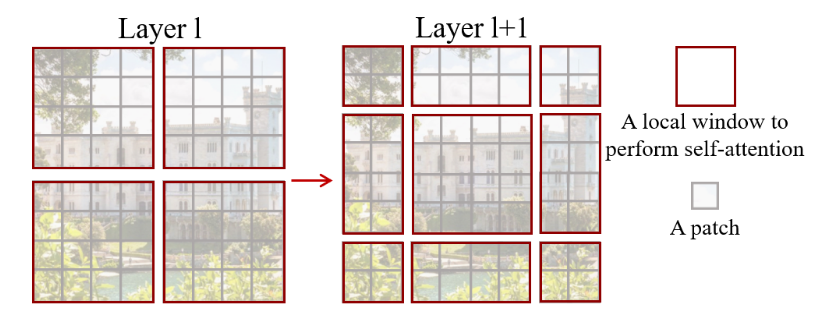
\includegraphics[width=\textwidth]{images/swin_shifted_window.png}}
	\caption{
	\textRL{طريقة النوافذ المزاحة بين كل كتلتين متعاقبتين في محول}
	\textLR{Swin}
	\textLR{\cite{swintransformer}}}
	\label{fig:swin_shifted_window}
\end{figure}
يبين الشكل
\ref{fig:swin_shifted_window}
كيفية اختيار تقسيم النوافذ من أجل كتلتين أو طبقتين متتاليتين من محول 
\textLR{Swin}.
الطبقة الأولى 
$l$
( الصورة اليسار) تقسم النوافذ بشكل نظامي، ويحسب الانتباه الذاتي ضمن أقسام النافذة الواحدة، كل نافذة على حدة.
الطبقة التالية من محول 
\textLR{Swin}
تقسم النوافذ بشكل مزاح عن نوافذ الطبقة السابقة، وذلك بمقدار نصف نافذة إلى جهة اليمين ونصف نافذة إلى الأسفل.
توضح المعادلات 
\ref{eq:swin_SW}
 خرج السمات من أجل كتلتين متعاقبتين لمحول 
\textLR{Swin} 
في مرحلة واحدة.
المعادلة الأولى تحسب الانتباه من أجل تقسيم النوافذ النظامي، الشكل
\ref{fig:swin_shifted_window}
 اليسار.
أما المعادلة الثالثة فهي حساب الانتباه ضمن النوافذ المزاحة، الشكل
\ref{fig:swin_shifted_window}
اليمين
\begin{equation}
	\begin{split}
	&\hat{z}^l = W-MSA(LN(z^{l-1}))+z^{l-1}\\
	&z^l = MLP(LN(\hat{z}^l))+\hat{z}^l\\
	&\hat{z}^{l+1} = SW-MSA(LN(z^l))+z^l\\
	&z^{l+1} = MLP(LN(\hat{z}^{l+1}))+\hat{z}^{l+1}\\
	\end{split}
	\label{eq:swin_SW}
\end{equation}
حيث 
$z_{l-1}$
خرج كتلة محول 
\textLR{Swin}
للمرحلة السابقة.
\subsubsection{تأثير النوافذ المزاحة وفائدتها}
نلاحظ أن النوافذ المزاحة في الطبقة 
$l+1$
تتقاطع مع نوافذ الطبقة 
$l$
ذات التقسيم النظامي، وهذا التقاطع يؤمن اتصال وتبادل معلومات بين النوافذ المجاورة كون الانتباه يحسب ضمن النافذة فقط، ويتجاهل النوافذ الأخرى.
طريقة النوافذ المزاحة قد حسنت من قدرة النمذجة للنموذج وهذا مايوضحه البحث 
\textLR{\cite{swintransformer}}
\subsubsection{الإزاحة الحلقية
\textLR{cyclic-shifting}}
ينتج عن طريقة النوافذ المزاحة زيادة في عدد النوافذ، بحيث لو كان عدد النوافذ في التقسيم النظامي
$\frac{h}{M} \mathsf{x} \frac{w}{M}$
يصبح في طبقة النوافذ المزاحة
$(\frac{h}{M} +1) \mathsf{x} (\frac{w}{M}+1)$،
حيث
$M \mathsf{x} M$
عدد أجزاء النافذة الواحدة. وكما في الشكل 
\ref{fig:swin_shifted_cycled_window}
 فإن بعض النوافذ سيكون حجمها أقل من 
$M\mathsf{x}M$.
أبسط طريقة لحل هذه المشكلة هي بحشو 
\textLR{pad}
النوافذ صغير الحجم لتصبح ببعد 
$M\mathsf{x}M$،
ومن ثم حساب الانتباه الذاتي داخل هذه النافذ  مع حجب القيم المحشوة.
هذا الحل لا يزيد من التعقيد الحسابي للنموذج حين يكون عدد النوافذ صغير، ولكن في حال العدد الكبير للنوافذ فقد اقترح النموذج طريقة الإزاحة الحلقية. 
\begin{figure}[!h]
	\centerline{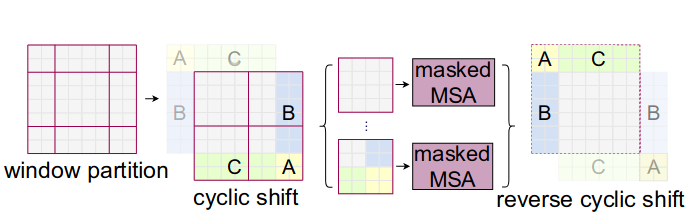
\includegraphics[width=\textwidth]{images/swin_shifted_cycled_window.png}}
	\caption{
		الازاحة الحلقية المستخدمة في محول
		\textLR{Swin}
		\textLR{\cite{swintransformer}}}
	\label{fig:swin_shifted_cycled_window}
\end{figure}
هذه الطريقة كما يوضح الشكل 
\ref{fig:swin_shifted_cycled_window}
 فإنه يتم إعادة ترتيب الأقسام بشكل حلقي حتى يكون عدد النوافذ متساوِ قبل وبعد الإزاحة. وأثناء إعادة الترتيب بشكل حلقي يمكن أن تحتوي النافذة على أجزاء من النوافذ الأخرى غير المجاورة لها،  ولحساب الانتباه الذاتي في هذه الحالة نستخدم تقنية الحجب 
\textLR{masking}
 وذلك لكي لا تدخل النوافذ غير المجاورة في حساب الانتباه الذاتي.
في هذه الحالة نحافظ على عدد النوافذ في حال التقسيم النظامي وفي حال التقسيم المزاح.
بينت التجربة في المقالة
\textLR{\cite{swintransformer}}
أن طريقة الازاحة الحلقية أسرع من طريق الحشو.
\begin{figure}[!h]
	\centerline{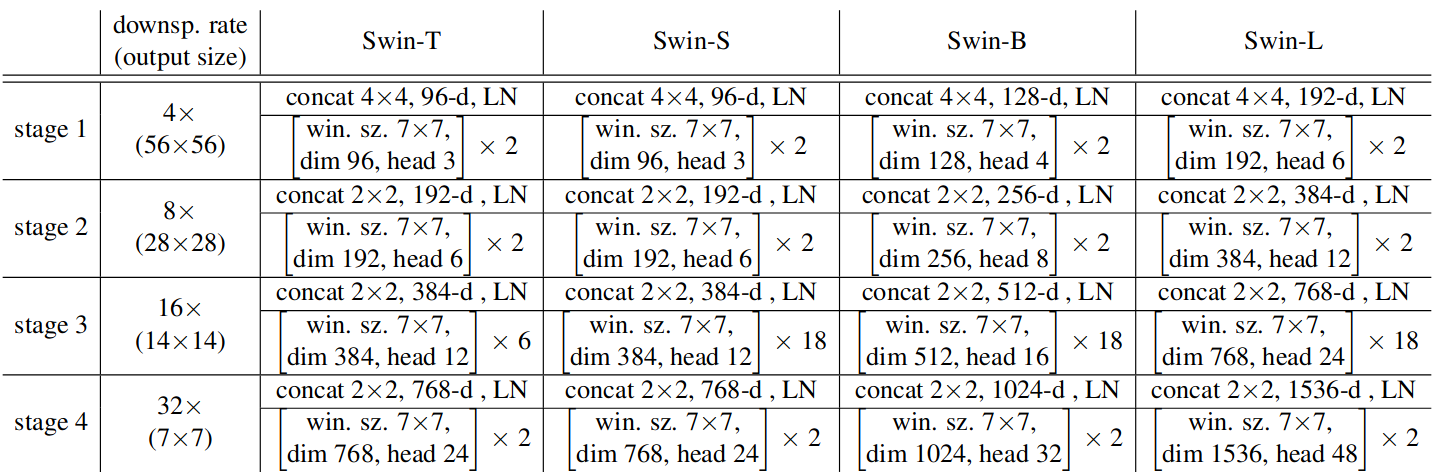
\includegraphics[width=\textwidth]{images/swin_architecture_table.png}}
	\caption{
	\textRL{أبعاد نموذج }
	\textLR{Swin}
	\textRL{من أجل عدة نسخ}
	\textLR{\cite{swintransformer}}}
	\label{fig:swin_architecture_table}
\end{figure}
يبين الجدول 
\ref{fig:swin_architecture_table}
أبعاد كل مرحلة من مراحل محول 
\textLR{Swin}
وذلك من أجل أبعاد مختلفة لصورة الدخل (السطر الأول من الجدول)، من أجل ملاحق
\textLR{Swin} 
فقد تم تدريبه من أجل عدة نسخ من المحول، اخترنا تطوير النسخة التي تستخدم
\textLR{Swin-Tiny}
كونه النموذج الأسرع والأقل كلفة في التدريب.
\section{خلاصة}
نستنتج من خلال الدراسة المرجعية بأن الاتجاه في تطوير نظم الملاحقة السائد يعتمد على التعلم العميق وخاصة نماذج المحول
ومن نتائج الشكل 
\ref{fig:comapre}
نلاحظ بأن خوارزميات الملاحقة ماتزال بحاجة إلى مزيد من البحث والتحسين من ناحية السرعة والأداء.
\section{خاتمة}
عرضنا في هذا الفصل مقدمة عن الملاحقة وأنواعها والمشكلات التي تواجها، وكان التركيز على أنواع ملاحقات التعلم العميق، إذ أن البحث يستهدف ملاحق 
\textLR{SwinTrack-Tiny\cite{swinTrack}}
الذي يعتمد على محول
\textLR{Swin\cite{swintransformer}}
لاستخلاص السمات، إذ أن تصميم هذه النسخة من المحول مناسب لتطبيقات الرؤية الصنعية كالملاحقة بسبب سرعة أداءه.
\\
تحدثناعن نموذج المحول وكيفية تطوره باستخدامه لتوابع الانتباه فقط وبذلك تجنب مشاكل الشبكات العودية، وقد تم شرح بنية المحول الأصلي مع التركيز على شرح تابع الانتباه، والذي استخدمناه لدمج سمات الصور في نموذجنا كما سنتحدث في الفصل القادم. وذكرنا تطبيقات المحول في الرؤية الحاسوبية، مع شرح مفصل لنموذج
\textLR{SwinTransformer}
وبينّا سبب استخدامنا له كونه مناسب لتطبيقات الرؤية الصنعية، إذ أنه أقل تعقيداً من نموذج المحول الأصلي في حال صورة دخل بأبعاد كبيرة.
وفي الفقرة الأخيرة تحدثنا عن تطبيقات المحول في  الملاحقة والتي بدأت منذ $2021$ .










